% Order matters.
% Document class.
%       Document types:
%             scrartcl: articles
%             scrreprt: longer articles
%             scrbook: books; allows \chapter for sections
%             scrlettr: letters
%       Paper formats:
%             default: US letter
%             a4paper: A4
%       Additional options
%             titlepage|notitlepage: use dedicated page for the title
%             onecolumn|twocolumn
%             oneside|twoside: one/two sided printing
%
\documentclass[12pt, a4paper]{report}



\usepackage[a4paper]{geometry}      % Paper format
\usepackage[OT2, T1]{fontenc}       % Font encoding. Displays fonts badly, unless ...
\usepackage{lmodern}                % ... this is enabled.
\usepackage[latin9]{inputenc}       % Input encoding.latin9 = Latin9/ISO-8859-15
\usepackage[english]{babel}         % english|ngerman (new german)



% Serif headlines for scr document classes
% Description: see page 61 (on \setkomafont) in the KOMA manual
% \setkomafont{sectioning}{\normalfont\bfseries}



% Header and footer
\usepackage{scrpage2}
\pagestyle{scrheadings}
\clearscrheadfoot
\usepackage{lastpage} % enables \pageref{LastPage}

%\automark[subsection]{section} % Creates an automark corresponding to the current section/subsection.
%\ihead{\headmark}
%\chead{}
%\ohead{\textnormal{\pagemark/\pageref*{LastPage}}}
%\ifoot{}
\cfoot{---~\pagemark~---}
%\ofoot{}
%\setheadsepline{.2mm} % Thin line below head



% Customize captions of figures etc.
\usepackage{caption}
\captionsetup{margin=1cm, indention=0cm}

% Indentation for figure captions
% \setcapindent{0mm}

% Names of figures, tables etc
% Note that \renewcommand\figurename alone doesn't work because of babel
\addto\captionsenglish{\renewcommand\figurename{Figure}}


% Chapter numbering
	% Section enumeration
	%       -1: nothing
	%       0-: Depth down to which is enumerated
	\setcounter{secnumdepth}{2}
	% Available numbered entities: \the... part, chapter, section, subsection, subsubsection, paragraph, subparagraph, page, equation, figure, table, footnote, mpfootnote, enumi, enumii, enumiii, enumiv
	% Available numbers (\command{counter}):
	%       \alph, \Alph: a-z, A-Z
	%       \arabic: 0-9
	%       \fnsymbol: Different special character for each counter
	%       \roman, \Roman: i, I
	\renewcommand{\thechapter}{\arabic{chapter}}
	\renewcommand{\thesection}{\arabic{chapter}.\arabic{section}}
	\renewcommand{\thesubsection}{\arabic{chapter}.\arabic{section}.\arabic{subsection}}
	\renewcommand{\theequation}{\arabic{section}.\arabic{equation}}


% Table of contents depth, similar to secnumdepth above.
% 0 = chapters
% 1 = sections
% ...
\setcounter{tocdepth}{2}
































 % Document class and layout
% AMS packages
\usepackage{amsmath, amssymb, amstext}



% Tensor package
% Full documentation: http://ftp.uni-erlangen.de/mirrors/CTAN/macros/latex/contrib/tensor/tensor.pdf
% Usage:
% Indices only: \indices{^a_{bc}}
% Tensor: \tensor[indices before]{tensor name}{indices after}
\usepackage{tensor}



% smashoperator
\usepackage{mathtools}



% Provides better support for underlined (etc) text. Use [normalem] to not alter \emph to underlining.
\usepackage[normalem]{ulem}



% Cancel package (strike-through formulas)
% Usage: \cancel{} \bcancel{} \xcancel{} \cancelto{}{}
\usepackage{cancel}



% Extended graphics support
\usepackage{graphicx}



% Colorizing things
% Usage: {\color{grey}lorem ipsum}
\usepackage{xcolor}
\definecolor{gray}{rgb}{0.6,0.6,0.6}
\definecolor{red}{rgb}{0.8,0,0}
\definecolor{green}{rgb}{0.04,0.62,0.14}



% Double strike font \mathds{}
\usepackage{dsfont}



% Script font \mathscr{}
\usepackage{mathrsfs}



% Hyperlinks, internal and external.
\usepackage{hyperref}
\hypersetup{
	% Color links
	colorlinks=true,
	citecolor=black,
	filecolor=black,
	linkcolor=black,
	urlcolor=black
}



% Create index.
% Create entry via \index{name[subname[subsubname]] (depth optional)
% Print using \printindex
\usepackage{makeidx} \makeindex



% Generate warnings when using deprecated commands
\usepackage[l2tabu, orthodox]{nag}



% Multicolumn sections.
% Example: Two-column layout: \begin{multicols}{2} lorem ipsum \end{multicols}
\usepackage{multicol}

% Enables lipsum text using \lipsum. \lipsum[i-j] prints paragraphs i to j. Maximum is 150.
\usepackage{lipsum}
\setlipsumdefault{1} % Print first paragraph by default



% Better date/time support
\usepackage{datetime}
\renewcommand{\dateseparator}{-}
\renewcommand{\timeseparator}{:}
\newcommand\Date{\the\year \dateseparator \twodigit\month \dateseparator \twodigit\day}
\newcommand\Time{\currenttime}


% Theorems
% amsmath = compatibility
% thmref = references to theorems
% hyperref = compatibility
% noconfig = don't load default theorem styles
% thmmarks = theorem end marks
\usepackage[amsmath, thref, hyperref, noconfig, thmmarks]{ntheorem} % (Way better than amsthm)
\theorembodyfont{\normalfont}
% Theorems
	\theoremstyle{break}
	\theoremheaderfont{\scshape}
	\newtheorem{theorem}{Theorem}%[section]
	\newtheorem{corollary}[theorem]{Corollary}
	\newtheorem{definition}[theorem]{Definition}
	\newtheorem{proposition}[theorem]{Proposition}
% Proof
	\theoremstyle{nonumberplain}
	\theoremheaderfont{\slshape}
	\theoremseparator{.}
	\theoremsymbol{\ensuremath{\square}}
	\newtheorem{proof}{Proof}
% Examples, remarks
	\theoremstyle{plain}
	\theoremheaderfont{\slshape}
	\theoremsymbol{\ensuremath{\bigtriangleup}}
	\theoremseparator{:}
	\newtheorem{example}{Example}%[section]
	\newtheorem{remark}[example]{remark}



































 % Additional packages
% Environments

% Math
\newcommand{\Equation}[1]{\begin{equation*}#1\end{equation*}}    % equation
\newcommand{\NEquation}[1]{\begin{equation}#1\end{equation}}     % equation (numbered)
\newcommand{\Align}[1]{\begin{align*}#1\end{align*}}             % block equation without numbering
\newcommand{\NAlign}[1]{\begin{align}#1\end{align}}              % block equation with numbering. Use \notag to suppress numbering locally.
%\newcommand{\Inline}[1]{\(#1\)}                                  % inline equation DEPRECATED.
% Sub-math
\newcommand{\Split}[1]{\begin{split}#1\end{split}}               % split (for use inside Align)
\newcommand{\Cases}[1]{\begin{cases}#1\end{cases}}               % piecewise functions etc (for use in math mode)
% Matrices
\newcommand{\Matrix}[1]{\begin{matrix}#1\end{matrix}}            % matrix without parentheses
\newcommand{\MatrixP}[1]{\begin{pmatrix}#1\end{pmatrix}}         % () matrix ("parentheses matrix")
\newcommand{\MatrixB}[1]{\begin{bmatrix}#1\end{bmatrix}}         % [] matrix ("braces matrix")
\newcommand{\MatrixC}[1]{\begin{Bmatrix}#1\end{Bmatrix}}         % {} matrix ("curly matrix")
\newcommand{\MatrixD}[1]{\begin{vmatrix}#1\end{vmatrix}}         % || matrix ("det matrix")
\newcommand{\MatrixN}[1]{\begin{Vmatrix}#1\end{Vmatrix}}         % || || matrix ("norm matrix")
% Quotes
\newcommand{\Qe}[1]{`#1'}                                        % quotes english
\newcommand{\Dqe}[1]{``#1''}                                     % double quotes english
\newcommand{\Qg}[1]{\glq{}#1\grq}                                % quotes german
\newcommand{\Dqg}[1]{\glqq{}#1\grqq}                             % double quotes german



% Abbreviations for common operations

% General
\renewcommand{\d}{\mathrm{d}}                                    % differential
\renewcommand{\i}{\mathrm{i}}                                    % imaginary unit
\renewcommand{\inf}{\infty}                                      % infinity
\newcommand{\infint}{\int_{-\inf}^\inf}                          % integral from -inf to inf
\newcommand{\inflint}{\int\limits_{-\inf}^\inf}                  % integral from -inf to inf with \limits
% Differential quotients
\newcommand{\tdq}[2]{\frac{\d #1}{\d #2}}                        % total differential quotient
\newcommand{\pdq}[2]{\frac{\partial #1}{\partial #2}}            % partial differential quotient
\newcommand{\vpdq}[1]{\frac{\vec\partial}{\vec\partial #1}}      % vector partial differential quotient
\newcommand{\vdq}[2]{\frac{\delta #1}{\delta #2}}                % variational differential quotient
% Frequent terms
\renewcommand\exp{\operatorname{exp}}                            % exp
\renewcommand\sin{\operatorname{sin}}                            % sin
\renewcommand\cos{\operatorname{cos}}                            % cos
\renewcommand\tan{\operatorname{tan}}                            % tan
\renewcommand\cot{\operatorname{cot}}                            % cot
\renewcommand\Re{\operatorname{Re}}                              % Re
\renewcommand\Im{\operatorname{Im}}                              % Im
\newcommand\Res{\operatorname*{Res}}                             % Res (* produces underset subscripts)
\renewcommand\div{\operatorname{div}}                            % div
\newcommand\grad{\operatorname{grad}}                            % grad
\newcommand\curl{\operatorname{curl}}                            % curl
\newcommand\rot{\operatorname{curl}}                             % rot = curl
\newcommand\sign{\operatorname{sign}}                            % sign
\renewcommand\deg{\operatorname{deg}}                            % degree
\newcommand\supp{\operatorname{supp}}                            % support
\newcommand\Tr{\operatorname{Tr}}                                % trace
\renewcommand\det{\operatorname{det}}                            % determinant
\newcommand\ind{\operatorname{ind}}                              % winding number
\newcommand\vol{\operatorname{vol}}                              % volume form
\newcommand\unity{\mathds{1}}                                    % identity matrix/operator
\newcommand\id{\operatorname{Id}}                                % identity
\newcommand\const{\mathrm{const.}}                               % Constants



% Redefinitions, fixing ambiguities
\newcommand\hodge{*}                                             % Hodge star
\newcommand\cross{\times}                                        % cross product
\renewcommand\vec[1]{\boldsymbol{#1}}                            % print vectors bold
\newcommand\laplace{\Delta}                                      % Laplace operator



% Special fonts
\newcommand\Cal[1]{\mathcal{#1}}                                 % Calligraphic (upper/lower case)
\newcommand\Frak[1]{\mathfrak{#1}}                               % Fraktur (upper/lower case)
\newcommand\Script[1]{\mathscr{#1}}                              % Script (upper case only)
\newcommand\Set[1]{\mathbb{#1}}                                  % Set/double stroke (upper case only)



% Units (m/s^2)
\newcommand{\Unit}[1]{\;\mathrm{#1}}



% References to different objects
\newcommand{\RefTheorem}[1]{\hyperref[#1]{\{\ref*{#1}\}}} % {123}
\newcommand{\RefEqn}[1]{\hyperref[#1]{(\ref*{#1})}} % (123)
\newcommand{\RefFigure}[1]{\hyperref[#1]{\ref*{#1}}} % 123
\newcommand{\RefSection}[1]{\hyperref[#1]{\ref*{#1}}} % 123



% Nicer square root
\def\nicesqrt{\mathpalette\DHLhksqrt}
\def\DHLhksqrt#1#2{%
\setbox0=\hbox{$#1\oldsqrt{#2\,}$}\dimen0=\ht0%
\advance\dimen0-0.2\ht0%
\setbox2=\hbox{\vrule height\ht0 depth -\dimen0}%
{\box0\lower0.4pt\box2}}



% Todo placeholder:
\newcommand{\TODO}[1]{{\color{red}[TODO: #1]}}



























 % Custom commands
% Cyrillic
% Syntax: \CYR#

\newcommand\cyrillic[1]{{\fontencoding{OT2}\fontfamily{wncyr}\selectfont #1}}
\newcommand\mathcyr[1]{\text{\cyrillic{#1}}}
                                                                % a     (identical to a)
                                                                % A     (identical to A)
\newcommand\CYRbe{\mathcyr{b}}                                  % be    (resembles delta)
\newcommand\CYRBe{\mathcyr{B}}                                  % Be    (resembles b)
\newcommand\CYRve{\mathcyr{v}}                                  % ve    (small B)
                                                                % Ve    (identical to B)
\newcommand\CYRge{\mathcyr{g}}                                  % ge    (small Gamma)
                                                                % Ge    (identical to Gamma)
\newcommand\CYRde{\mathcyr{d}}                                  % de    (somewhat edgy-A-looking)
\newcommand\CYRDe{\mathcyr{D}}                                  % De    (larger version of de)
                                                                % ye    (identical to e)
                                                                % Ye    (identical to E)
\newcommand\CYRzhe{\mathcyr{zh}}                                % zhe   (resembles asterisk)
\newcommand\CYRZhe{\mathcyr{Zh}}                                % Zhe   (larger version of zhe)
                                                                % dze   (identical to s)
                                                                % Dze   (identical to S)
                                                                % ze    (almost identical to 3)
                                                                % Ze    (larger version of ze)
\newcommand\CYRinvn{\mathcyr{i}}                                % -     (inverted N)
\newcommand\CYRInvn{\mathcyr{I}}                                % -     (larger version of invn)
                                                                % k     (identical to kappa)
                                                                % K     (identical to Kappa)
\newcommand\CYRel{\mathcyr{l}}                                  % el    (resembles pi)
\newcommand\CYREl{\mathcyr{L}}                                  % El    (resembles Pi)
\newcommand\CYRemm{\mathcyr{m}}                                 % em    (small M)
                                                                % Em    (identical to M)
\newcommand\CYRen{\mathcyr{n}}                                  % en    (small N)
                                                                % En    (identical to N)
                                                                % o     (identical to o)
                                                                % O     (identical to O)
\newcommand\CYRpe{\mathcyr{p}}                                  % pe    (small Pi)
                                                                % Pe    (identical to Pi)
                                                                % koppa (identical to c)
                                                                % Koppa (identical to C)
                                                                % er    (identical to p)
                                                                % Er    (identical to P)
\newcommand\CYRte{\mathcyr{t}}                                  % te    (small T)
                                                                % Te    (identical to T)
                                                                % tshe  (identical to hbar)
\newcommand\CYRTshe{\mathcyr{C1}}                               % Tshe  (T+h)
                                                                % ef    (almost identical to varphi)
                                                                % Ef    (identical ti Phi)
                                                                % kha   (identical to x)
                                                                % Kha   (identical to X)
\newcommand\CYRtse{\mathcyr{ts}}                                % tse   (small upside-down Pi with some kind of a hook)
\newcommand\CYRTse{\mathcyr{Ts}}                                % Tse   (larger version of tse)
\newcommand\CYRche{\mathcyr{ch}}                                % che   (turn h by 180)
\newcommand\CYRChe{\mathcyr{Ch}}                                       % Che   (larger version of che)
\newcommand\CYRsha{\mathcyr{sh}}                                % sha   (small upside-down triple pi)
\newcommand\CYRSha{\mathcyr{Sh}}                                % Sha   (larger version of sha)
\newcommand\CYRshta{\mathcyr{shch}}                             % shta  (sha with hook)
\newcommand\CYRShta{\mathcyr{Shch}}                             % Shtaa (Sha with hook)
\newcommand\CYRyer{\mathcyr{p2}}                                % yer   (hard sign, small b with a hook)
\newcommand\CYRYer{\mathcyr{P2}}                                % Yer   (larger version of yer)
                                                                % yeri  (bI. that's two characters. gtfo.)
                                                                % yat   (more b with more hooks, no, i'm out)
\newcommand\CYRyu{\mathcyr{yu}}                                 % yu    (|-O)
\newcommand\CYRYu{\mathcyr{Yu}}                                 % Yu    (larger version of yu)
\newcommand\CYRya{\mathcyr{ya}}                                 % ya    (mirrored R)
\newcommand\CYRYa{\mathcyr{Ya}}                                 % Ya    (larger version of ya)
% Test all letters:
% \be\Be\ve\ge\de\De\zhe\Zhe\invn\Invn\el\El\em\en\pe\te\Tshe\tse
% \Tse\che\Che\sha\Sha\shta\Shta\yer\Yer\yu\Yu\ya\Ya % Cyrillic letters
% TikZ
\usepackage{tikz}
\usetikzlibrary{
	arrows,
	backgrounds,
	calc,
	decorations.markings,
	decorations.pathmorphing,
	fit,
	intersections,
	patterns,
	positioning,
	through
}

% Arc around a point
\newcommand\TikzArcAround[3]{
	% #1: radius
	% #2: start angle
	% #3: delta angle
	% Example: \draw (1,0) \ArcAround{2}{60}{120}
	++(#2:#1)
	arc[radius=#1, start angle=#2, delta angle=#3]
}

% Helper coordinate system
\newcommand\TikzCoSy[4]{
	% Arguments: integers: x1, x2, y1, y2 ("x range, y range")
	% Lower numbers first!
	(#1,#3) grid (#2,#4)
}
\newcommand\TikzCoSyLabels[4] {
	\foreach \x in {#1,...,#2} {
		node at (\x,0) {\x}
	}
	\foreach \y in {#3,...,#4} {
		\ifnum \y = 0
		\else
			node at (0,\y) {\y}
		\fi
	}
}
\newcommand\TikzFullCoSy[4] {
	\TikzCoSy{#1}{#2}{#3}{#4}
	\TikzCoSyLabels{#1}{#2}{#3}{#4}
}

% Draws a cross at the current location with radius #1.
\newcommand\TikzCross[1]{
	% 0.707107/2 = 1/sqrt(2) for the rotation to get the "x" shape
	+( #1/0.707107/2, #1/0.707107/2) -- +(-#1/0.707107/2,-#1/0.707107/2)
	+( #1/0.707107/2,-#1/0.707107/2) -- +(-#1/0.707107/2, #1/0.707107/2)
	+(0,0)
}

\newcommand\TikzClipMask{
	\draw [draw=black, fill=orange, opacity=0.5, draw opacity=0.8]
}

% Useful for decorations.
% Example:
% mark=between positions 0.0 and 1.0 step 0.1 with {\node (node\pgfkeysvalueof{\SequenceNumber}) [label=below right:{$y_\pgfkeysvalueof{\SequenceNumber}$}] {};}
% Adds nodes named "nodeX" at evenly spaced intervals to a path.
\newcommand\SequenceIndex{\pgfkeysvalueof{/pgf/decoration/mark info/sequence number}}

% Parse mathematical expressions
\newcommand\TikzMath[1] {
	\pgfmathparse{#1}
	\pgfmathresult
}

% Use stealth arrowheads as default
\tikzstyle{every picture}+=[>=stealth]


% Draw arrow at arbitrary position using ->-=0.5 etc
\tikzset{->-/.style={decoration={
	markings,
	mark=at position #1 with {\arrow{>}}},postaction={decorate}}}












     % Drawing figures


\title{Foobar}
\author{David Luposchainsky}

\newcommand\SEnv{\ensuremath{S_\text{env}}}
\newcommand\STot{\ensuremath{S_\text{tot}}}
\newcommand\SSys{\ensuremath{S_\text{sys}}}
\newcommand\SF{\text{SF}}
\newcommand\HF{\text{HF}}

\newcommand\Ito{It\=o}
\newcommand\init{\text{init}}

% Mathematica's first four ColorData[81] colors:
\definecolor{blue}{rgb}{0, 0.26, 0.5}
\definecolor{yellow}{rgb}{0.9, 0.648, 0}
\definecolor{red}{rgb}{0.75, 0, 0}
\definecolor{cyan}{rgb}{0, 0.6, 0.6}
% Others
\definecolor{lgray}{rgb}{0.85, 0.85, 0.85}

% Change headline styles
\usepackage{titlesec}
\titleformat{\chapter}
	{\normalfont\Huge\bfseries\color{blue}}{\thechapter}{1em}{}
\titleformat{\section}
	{\normalfont\Large\bfseries\color{blue}}{\thesection}{1em}{}
\titleformat{\subsection}
	{\normalfont\large\bfseries\color{blue}}{\thesubsection}{1em}{}
\titleformat{\subsubsection}
	{\normalfont \bfseries\color{blue}}{\thesubsubsection}{1em}{}

\begin{document}



\titlepage
\vspace*{1em}
\begin{center}
	\LARGE{\bfseries
		Production and fluctuation of environmental entropy
	}

	\vfill %\vspace{1.5cm}

	\begin{center}
		
\includegraphics[width=0.4\textwidth]{figures/unilogo.pdf}
	\end{center}

	\vfill %\vspace{1.5cm}

	\Large{Master thesis in physics}\\

	\vfill

	{\Large David Luposchainsky} \\ [0.5 cm]
	Supervised by\\
	{\Large Prof. Dr. Haye Hinrichsen}

	\vfill

	W�rzburg 2012-13

\end{center}

\tableofcontents

\chapter{Introduction}

explain master equation in the thingie chapter


\section{Historical overview}

\section{Entropy}

Shannon entropy

Popsci explanations

Zwiebelfisch

Entropie eines einzelnen Teilchens erkl�ren


``Taking away the averages''


\section{Thesis overview}

This thesis is divided in two parts, the first one being about environmental entropy in a discrete, the second one in a continuous setting. Although both parts are independent research subjects, they do share certain ideas and definitions. For this reason some issues in chapter~\ref{chap:flow} are assumed to be known due to being introduced in chapter~\ref{chap:thingie}. Both of these chapters will provide their own overviews at the beginning.


\subsection{A new set of fluctuation theorems}

Chapter~\ref{chap:thingie} is the result of modifying computer simulation, leading to a surprising outcome: when the resulting histogram was weighted using a seemingly arbitrary factor, it turns out to obey a certain symmetry called detailed fluctuation theorem. A detailed fluctuation theorem is an equation of the form
%
\begin{equation}
	p(x) = e^{x}p(-x)
\end{equation}
%
that is fulfilled by a distribution \(p\) for all values \(x\).

This distribution will be the likelihood to obtain a certain value of one special form of entropy, for which no fluctuation theorems were previously known. Deeper investigation of the phenomenon lead to the discovery of an entire new class of fluctuation theorems, and as a possible application a model for how sudden temperature changes affect the energy flow from/to the environment of a simple system.





\subsection{Entropy in continuous settings}

The second topic is discussed in chapter~\ref{chap:flow}, which is concerned with how entropy can be defined in a meaningful way in a continuous setting. This is surprisingly difficult, as one could naively think the definitions just carry over. To give a motivating example, consider the before mentioned definition of entropy for a discrete distribution,
%
\begin{equation}
	S_\text{discrete} = \sum_ip_i\ln p_i
\end{equation}
%
and make it continuous by scaling down the intervals over which \(p\) changes its value. In the limit this will result in an integral of the form
%
\begin{equation}
	S_\text{cont.} = \int_\Omega\d x\,p(x)\ln p(x) ~.
\end{equation}
%
But there is a problem with this equation: it does not have a lower bound. Intuitively, the \(\delta\)~distribution should have no entropy, as it is the continuous version of a single-valued state. However, inserting it into the equation above results in \(S = -\infty\). Take \(\Omega = \Set R\) and a Gaussian with zero mean and standard deviation \(\sigma\), insert everything in the above equation, then the result will be
%
\begin{align}
	p_\sigma(x) &= \frac1{\sqrt{2\pi\sigma^2}} \exp\left(-\frac{x^2}{2\sigma^2}\right) \\
	\Rightarrow S_\text{cont.} &= -\ln(\sigma) + \const
\end{align}
%
which is logarithmically divergent for \(\sigma\to0\), the same limit that yields the \(\delta\)~distribution for a Gaussian. Another way of looking at it is that a \(\delta\) centered at a real value \(\mu\) carries infinite information (hence infinite entropy), namely all the decimals of \(\mu\); in a discrete setting, that would merely be an integer.

This was but one motivating example. The actual work in chapter~\ref{chap:flow} will be concerned with how the concept of environmental entropy -- in many cases easier to picture as the heat exchange with the environment -- can be brought from its easy discrete definition into a setting where the degrees of freedom are continuous.






% Strong fluctuation theorem for S_env
\chapter{Strong fluctuation theorem for environmental entropy}
\label{chap:thingie}

The contents of this chapter were published in Physical Review E, ``Strong fluctuation theorem for nonstationary nonequilibrium systems'' \cite{thingie-paper}. The following is an elaborate description of its contents.

This chapter has two main parts. The first one provides an introduction to fluctuation theorems, Markov processes, entropy, and the terminology used. The secone one then uses these definitions to prove a new general fluctuation theorem, specializes it to appear in a more familiar form, and finally puts it to the test in two numerical examples.


%%%%%%%%%%%%%%%%%%%%%%%%%%%%%%%%%%%%%%%%%%%%%%%%%%%%%%%%%%%%%%%%%%%%%%%%%%%%%%
\section{Preliminaries}
%%%%%%%%%%%%%%%%%%%%%%%%%%%%%%%%%%%%%%%%%%%%%%%%%%%%%%%%%%%%%%%%%%%%%%%%%%%%%%



%%%%%%%%%%%%%%%%%%%%%%%%%%%%%%%%%%%%%%%%%%%%%%%%%%%%%%%%%%%%%%%%%%%%%%%%%%%%%%
\subsection{Fluctuation theorems}
%%%%%%%%%%%%%%%%%%%%%%%%%%%%%%%%%%%%%%%%%%%%%%%%%%%%%%%%%%%%%%%%%%%%%%%%%%%%%%

Classical thermodynamics is a theory of averages of certain quantities. For example, temperature is a measure for the \emph{mean} energy per degree of freedom of a gas, or the \emph{mean} cost of energy to increase the \emph{mean} entropy by a certain amount. Unfortunately, this approach requires certain quantities to exist a priori, and does not explain their origins. On the other hand, statistical physics typically starts with all individual constituents at the same time, and tries to explain how certain statistical properties -- the mean being just one of them -- emerge. In that sense, fluctuation theorems are about \textbf{taking away the averages} of classical thermodynamics. One of these averages is the entropy of a system \TODO{ref zum Vorspann}, of which we know that it obeys the second law of thermodynamics, typically written as
%
\begin{equation}
	\label{eqn:2nd_law_classical}
	\d S \geq 0 ~,
\end{equation}
%
meaning that thermodynamic (macroscopic) entropy is always increasing.

However, looking at the microscopic properties of a system, it is indeed possible that entropy spontaneously decreases -- when all microstates occur with some nonzero probability, there is also always a nonzero (albeit small) chance of transition to a highly ordered system. Fluctuation theorems provide a characteristic expression for the likelihood for certain statistical events to occur in a system. For example in the case of microscopic total entropy changes \(\Delta S\), it can be shown that
%
\begin{equation}
	P(\Delta S) = e^{\Delta S}P(-\Delta S)
\end{equation}
%
which states that the probability of spontaneous entropy increase by \(\Delta S\) is exponentially more likely than a decrease by the same amount; theorems of the above form will be referred to as \textbf{detailed} fluctuation theorems, as the expression yields symmetry information for each point of a distribution individually. In a sense, this is the analogon to the Second~Law from the viewpoint of statistical physics, and indeed it can be shown that \RefEqn{eqn:2nd_law_classical} can be recovered from this formula: integrating both sides yields
%
\begin{equation}
	\label{eqn:average of exp}
	1 = \inflint \d (\Delta S) P(\Delta S) = \inflint \d (\Delta S) e^{\Delta S}P(-\Delta S) = \left\langle e^{-\Delta S} \right\rangle
\end{equation}
%
which, using Jensen's inequality \(\langle e^x\rangle \geq e^{\langle x\rangle}\), implies
%
\begin{equation}
	\langle\Delta S\rangle \geq 0 ~.
\end{equation}
%
Averages of this form are known as \textbf{integral} fluctuation theorems.

It turns out that this derivation was overly general: in fact, a detailed fluctuation theorem implies arbitrarily many integral fluctuation theorems, since
%
\begin{align}
	   B
	&\equiv \langle e^{-\frac x2}A(x)\rangle
	= \inflint\d x \, P(x) e^{-\frac x2}A(x)
	= \int\limits_\infty^{-\infty}\d(-x) P(-x) e^{\frac x2}A(-x) \notag \\
	&= - \inflint\d x \, P(x) e^{-\frac x2}A(x)
	 = -B
	 = 0 \notag \\
	\label{eqn:antisymmetric exp average}
	&\Rightarrow
	\langle e^{-\frac x2}A(x)\rangle = 0
\end{align}

%
where \(A\) is an arbitrary antisymmetric function; the relation \RefEqn{eqn:average of exp} can be recovered by setting \(A(x) = \sinh(x/2) = \frac12(e^x-e^{-x})\).

This was but one example of a fluctuation theorem for \(\Delta S\); there are many more for other quantities (such as different forms of heat, work, other sub-categories of entropy), as can be seen e.g. in \cite{seifert-review}, and one of the main results of this chapter will be yet another entire class of fluctuation theorems.


%%%%%%%%%%%%%%%%%%%%%%%%%%%%%%%%%%%%%%%%%%%%%%%%%%%%%%%%%%%%%%%%%%%%%%%%%%%%%%
\subsection{Markov jumping processes}
\label{sec:markov process}
%%%%%%%%%%%%%%%%%%%%%%%%%%%%%%%%%%%%%%%%%%%%%%%%%%%%%%%%%%%%%%%%%%%%%%%%%%%%%%

A \emph{jumping process} is a system consisting of a discrete number of states that, governed by certain transition rates or probabilities, switches from one state to another repeatedly. A \emph{Markov process} is a special jumping process where the ``next'' state can only depend on the current state, and has no knowledge about its history. In other words, a Markov process is one in which the system does not have a concept of ``momentum'' in the colloquial sense.

An example for a jumping process is a gambler in a casino, the state being how much money he has. Each time he places a bet, he changes his state (loses or wins money).
%
\begin{enumerate}
	\item A realistic gambler can be seen jumping process, and can make his bets dependent on e.g. whether he lost his last game (which requires to know about the current balance and the one before that), or if he is suspicious kind could alter the winning probabilities in his favour. Note that the concept of ``winning streaks'' also falls into this category, as ``having'' one requires knowledge of the previous games/balances.
	\item A Markovian gambler would decide how much to bet based solely on how much money he currently has (and possibly how late it is). He would base none of his decisions on his knowledge about previous games.
\end{enumerate}






%%%%%%%%%%%%%%%%%%%%%%%%%%%%%%%%%%%%%%%%%%%%%%%%%%%%%%%%%%%%%%%%%%%%%%%%%%%%%%
\subsection{Terminology}
%%%%%%%%%%%%%%%%%%%%%%%%%%%%%%%%%%%%%%%%%%%%%%%%%%%%%%%%%%%%%%%%%%%%%%%%%%%%%%

Suppose we have a system \(\Omega\) of \(N\) states, enumerated by \(j\). Time runs from \(t = 0\) to \(t = T\). At times \(\tau_j\), the system transitions from an old state \(n_{j-1}\) into a new one. \(c_j\). Grouping multiple successive state changes together, we can describe the history of the system using a trajectory through time/state space with \(J\) jumps,
%
\begin{align}
	\gamma &=~
	\newcommand\iarrow[1]{~\underset{\tau_{#1}}\longrightarrow~}
	%
	c_0
	\iarrow{1}
	c_1
	\iarrow{2}
	\cdots
	\iarrow{j}
	c_{j}
	\iarrow{j+1}
	c_{j+1}
	\iarrow{j+2}
	\cdots
	\iarrow{J}
	c_{J}
	\\
	&= \{c_{i,\tau_i}\}
\end{align}
%
An ``element'' \(c_{i,\tau_i}\) of \(\gamma\) can thus be interpreted as ``the system is in state \(c_i\) starting at time \(\tau_{i}\), until \(\tau_{i+1}\)''. A visualization of the above description can be found in \RefFigure{fig:discrete_jumping_process}.

\begin{figure}[htb]
	\centering
	\begin{tikzpicture}
	[>=stealth]

	% coordinate system
	\begin{scope}
		% axes
		\begin{scope}[->]
			\newcommand\Excess{0.2}
			\draw (-\Excess,0) -- (10.5,0); % x
			\draw (0,-\Excess) -- (0,6);  % y
		\end{scope}


		\newcommand{\TickLength}{0.2}
		\newcommand{\LabelOffset}{0.5}
		
		% y axis labels/ticks
		\begin{scope}
			\foreach \y in {1,...,5} {
				\draw (-\TickLength/2, \y) -- (\TickLength/2, \y);
 				\node at (-\LabelOffset, \y) {\(\y\)};
			}
			\node at (0, 6 + \LabelOffset) {\(\Omega\)};
		\end{scope}

		% x axis labels/ticks
		\begin{scope}
			\foreach \i/\x in {0/0, 1/2, 2/3, 3/6, 4/7.5, 5/8, 6/10} {
				\draw (\x, -\TickLength/2) -- (\x, \TickLength/2);
				\node at (\x, -\LabelOffset) {\(\tau_\i\)};
			}
			\node at (0, -2*\LabelOffset) {\(0\)};
			\node at (10, -2*\LabelOffset) {\(T = \tau_{J+1}\)};

			\node at (10.5 + \LabelOffset, 0) {\(t\)};
		\end{scope}

	\end{scope}

	% Path taken
	\begin{scope}
		
		% Actual path
		\begin{scope} [thick]
			\draw (0,1) -- (2,1)
				(2,4) -- (3,4)
				(3,3) -- (6,3)
				(6,5) -- (7.5,5)
				(7.5,1) -- (8,1)
				(8,2) -- (10,2)
				;
			\newcommand{\Radius}{0.03}
			\foreach \xy in {(0,1), (2,1), (2,4), (3,4), (3,3), (6,3), (6,5), (7.5,5), (7.5,1), (8,1), (8,2), (10,2)} {
				\draw[fill=black] \xy circle (\Radius);
			}
		\end{scope}

		% Connecting jump lines
		\begin{scope} [dotted]
			\draw (2,1)-- (2,4)
			      (3,4) -- (3,3) 
				(6,3) -- (6,5) 
				(7.5,5) -- (7.5,1) 
				(8,1) -- (8,2)
				;
		\end{scope}

		% labels
		\begin{scope}
			\newcommand{\LabelOffset}{0.5}
			\node at (1,         1 - 0.5*\LabelOffset) {\small \(c_0 = 1\)};
			\node at (2.5,       4 + 0.5*\LabelOffset) {\small \(c_1 = 4\)};
			\node at (4.5,       3 - 0.5*\LabelOffset) {\small \(c_2 = 3\)};
			\node at (6.75,      5 + 0.5*\LabelOffset) {\small \(c_3 = 5\)};
			\node at (7.75,      1 - 0.5*\LabelOffset) {\small \(c_4 = 1\)};
			\node at (9,         2 + 0.5*\LabelOffset) {\small \(c_5 = 2\)};
		\end{scope}

		% final dashed line at t=T

		\begin{scope}
			\draw [dashed] (10,0) -- (10,6);
		\end{scope}
		
	\end{scope}

\end{tikzpicture}

	\caption[]{Visualization of a discrete jumping process with \(J = 5\) jumps. The system, initially in state \(c_0\) at time \(t = \tau_0 = 0\), transitions into a new state \(c_1\) at time \(\tau_1\), and remains in this state until the next jump occurs. The process then repeats itself, and the resulting trajectory is a representation of the system's history.}
	\label{fig:discrete_jumping_process}
\end{figure}

In a typical system, many such paths can be taken when starting from an initial configuration \(c_0\); depending on the dynamics of the system, the jumps can occur at different times or to different states. Due to the stochastic nature of the system, trajectories most likely occur with different probabilities; these probabilities will be denoted \(p[\{c_{i,\tau_i}\}|c_0]\) with an explicit mentioning of the starting point \(n_0\).



A Markov process on a set of \(N\) states is characterized by a (possibly time-dependent) transition matrix \(w_{c\to c'}\), whose entries are the rates at which the system jumps from one configuration \(c\) to another one \(c'\). Since later calculations will require ratios of rates it is required that in case of a nonzero jumping rate, the reverse jump also has a nonzero entry. Letting this system run for a certain amount of time will result in such a stochastic trajectory \(\gamma\) through the state space, and such trajectories are what this chapter is about.

Given such a process, the probability of a path \(p[\{c_{i,\tau_i}\}|c_0]\), containing a total of \(J\) jumps (and consequently covering intermediate \(J+1\) states), can be expressed as a series of ``staying in the same state'' and ``change state'' contributions \cite{seifert-review},
%
\begin{equation}
	\begin{split}
	\label{eqn:discrete path probability}
	p[\{c_{i,\tau_i}\} | c_0]
	& = \exp\left(-\int_{\tau_0}^{\tau_1}\d\tau\;r_{c_0}(\tau)\right)
	\\ &\qquad \times
	\prod_{j=1}^J
		w_{c_{j-1}\to c_j}(\tau_j)
		\exp\left(-\int_{\tau_j}^{\tau_{j+1}}\d\tau\;r_{c_j}(\tau)\right)
	\end{split}
\end{equation}
%
where \(r_c\) stands for the escape rate from state \(c\),
%
\begin{equation}
	r_c = \sum_{c'\neq c} w_{c\to c'} ~.
\end{equation}
%
Here the first line, \(\exp\left(-\int_{\tau_0}^{\tau_1}\d\tau\;r_{c_0}(\tau)\right)\), corresponds to the probability for staying in configuration \(c_0\) from time \(\tau_0\) to \(\tau_1\). This is then followed by a transition to \(c_1\) given by the first factor of the product, namely \(w_{\cdots}\), followed by staying in this configuration for times \(\tau_1\) to \(\tau_2\). The process -- jumping, then staying -- then repeats itself another \(J-1\) times, until all jumps have happened and the trajectory has been run through. The product of the probabilities of the constituents then makes up the overall path probability.

Assuming time-independent rates \(w\), the integrals in \RefEqn{eqn:discrete path probability} can trivially be evaluated, and the expression reduces to
\begin{equation}
	p[\{c_{i,\tau_i}\} | c_0]\Bigr|_{w\;\const}
	\equiv
	Q[\gamma]
	=
	e^{-(\tau_1-\tau_0)r_{c_0}} \left(
		\prod_{j = 1}^J
		w_{c_{j-1}\to c_j}
		e^{-(\tau_{j+1}-\tau_j)r_j}
		\right)
\end{equation}

It will also be necessary to calculate the probability of taking the steps of a path in reverse direction, denoted ``\(\dagger\)'', and the above definitions turn out as follows in this case:
%
\begin{align*}
	\gamma^\dagger &=~
	\newcommand\iarrow[1]{~\underset{T-\tau_{#1}}\longrightarrow~}
	%
	c_{J}
	\iarrow{J}
	\cdots
	\iarrow{j+2}
	c_{j+1}
	\iarrow{j+1}
	c_{j}
	\iarrow{j}
	\cdots
	\iarrow{2}
	c_1
	\iarrow{1}
	c_0
	\\
	&= \{c_{i,\tau_i}\}^\dagger
\end{align*}
%
\begin{equation}\begin{split}
	p^\dagger[\{c_{i,\tau_i}\}^\dagger | c_0^\dagger]
	&= \exp\left(-\int_{\tau_{J+1}}^{\tau_J}\d(-\tau)r_{c_J}(\tau)\right)
		\\&\qquad\times
		\prod_{j=J}^1
			w_{c_j\to c_{j-1}}(\tau_j)
			\exp\left(-\int_{\tau_j}^{\tau_{j-1}}\d(-\tau)r_{c_{j-1}}(\tau)\right)
	\\
	&= \exp\left(-\int_{\tau_J}^{\tau_{J+1}}\d\tau\;r_{c_J}(\tau)\right)
		\\&\qquad\times
		\prod_{j=1}^J
			w_{c_j\to c_{j-1}}(\tau_j)
			\exp\left(-\int_{\tau_{j-1}}^{\tau_j}\d\tau\;r_{c_{j-1}}(\tau)\right)
\end{split}\end{equation}

\begin{equation}
	p^\dagger[\{c_{i,\tau_i}\}^\dagger | c_0^\dagger]\Bigr|_{w\;\const}
	\equiv
	Q[\gamma^\dagger]
	=
	e^{-(\tau_{J+1}-\tau_J)r_{c_J}} \left(
		\prod_{j = 1}^J
		w_{c_j\to c_{j-1}}
		e^{-(\tau_j-\tau_{j-1})r_{j-1}}
		\right)
\end{equation}











%%%%%%%%%%%%%%%%%%%%%%%%%%%%%%%%%%%%%%%%%%%%%%%%%%%%%%%%%%%%%%%%%%%%%%%%%%%%%%
\subsection{Entropy in a Markov process}
%%%%%%%%%%%%%%%%%%%%%%%%%%%%%%%%%%%%%%%%%%%%%%%%%%%%%%%%%%%%%%%%%%%%%%%%%%%%%%

For Markov processes, it is often suitable not to look at the total entropy \STot{}, but to split it up in two constituents, namely the system entropy \SSys{} and the environmental entropy \SEnv{}.

The \textbf{system entropy} \(\mathbf{\SSys{}}\) is the Shannon entropy of an ensemble. Running a Markov process, starting with some random initial configuration \(c_0\) drawn using some distribution \(p_0(t=0)\), then after some time \(\Delta t\) the system will be in a new configuration \(c_i\). Repeating the procedure many times will yield a distribution \(p_i(t)\) of the various \(c_i\) reached. \SSys{} is now the Shannon entropy associated to that distribution:
%
\begin{align}
	\SSys(t) = \sum_i p_i(t)\ln p_i(t)
\end{align}
%
The standard interpretation of this relationship is that \SSys{} is a quantity describing how ``concentrated'' the system is around certain states at a single point in time, or in other words how much more likely it is to be in some specific state (or set of states) compared to others. For example, if the transition matrix \(w_{c\to c'}\) has a bias to make the system go into a particular subset of configurations, \SSys will be lower, while maximum entropy is achieved when all states are reached with the same probability.

On the other hand, the \textbf{environmental entropy} \(\mathbf{\SEnv{}}\) takes not the system's internal configuration into account, but characterizes how the current configuration has been reached. Each time the system changes its state, \SEnv{} increases by a certain amount,
%
\begin{align}
	\label{eqn:SEnv single jump definition}
	\Delta\SEnv^{c\to c'} = \ln\frac{w_{c\to c'}}{w_{c'\to c}} ~.
\end{align}
%
This provides a characteristic quantity for the reversibility of a process: \(\Delta \SEnv\) is zero if the jumps and its reverse are equally likely, larger than zero if a transition was made in a more likely state, and lastly smaller than zero if an unlikely jump happens.

A stochastic trajectory \(\gamma\) now is a series of many such jumps, hence the total of the accumulated environmental entropy can be seen as a functional on \(\gamma\),
%
\begin{align}
	\label{eqn:SEnv rate jump functional}
	\Delta\SEnv[\gamma] = \sum_{i=1}^J\ln\frac{w_{c_{i-1}\to c_i}}{w_{c_i\to c_{i-1}}}
\end{align}
%
where \(J\) is the total number of jumps in \(\gamma\), and \(c_i\) are the configurations it consists of.




%%%%%%%%%%%%%%%%%%%%%%%%%%%%%%%%%%%%%%%%%%%%%%%%%%%%%%%%%%%%%%%%%%%%%%%%%%%%%%
\subsection{Master equation}
\label{sec:master equation}
%%%%%%%%%%%%%%%%%%%%%%%%%%%%%%%%%%%%%%%%%%%%%%%%%%%%%%%%%%%%%%%%%%%%%%%%%%%%%%

One way of exploring the properties of a Markov process is to collect statistics via running the same experiment many times. Another approach is starting with the statistics in the first place -- instead of starting with individual processes and measuring their distribution, take the distribution of states and ask how it will evolve. This is what the \emph{Master equation} describes:
%
\begin{align}
	\label{eqn:master}
	\dot p_c(t)
		&= \underbrace{\sum_{c'} j_{c'\to c}}_{\text{gain}}
		- \underbrace{\sum_{c'} j_{c\to c'}}_{\text{loss}} \\
		&= \sum_{c'} p_{c'}(t)w_{c'\to c}
		- \sum_{c'} p_c(t)w_{c\to c'}
\end{align}
%
The first term describes the system jumping into a state (probability current \(j\) towards the state \(c\)), while the second one accounts for transitions out of it (current away from \(c\)). A stationary Master equation (\(\dot p \equiv 0\)) is characteristic for systems for which macroscopic quantities are constant, as described below.






%%%%%%%%%%%%%%%%%%%%%%%%%%%%%%%%%%%%%%%%%%%%%%%%%%%%%%%%%%%%%%%%%%%%%%%%%%%%%%
\subsection{Detailed balance}
\label{sec:detailed balance}
%%%%%%%%%%%%%%%%%%%%%%%%%%%%%%%%%%%%%%%%%%%%%%%%%%%%%%%%%%%%%%%%%%%%%%%%%%%%%%

When talking about a system obeying statistical dynamics, there is a certain hierarchy of names describing how ``equilibriated'' it is. In a general setting it cannot be assumed that a system obeys special statistical properties because it follows arbitrary dynamics, and is called being in total nonequilibrium. The other end of the spectrum is equilibrium, where all macroscopic properties of the system are constant. There are a few important intermediate notions though, and one of them is called \emph{detailed balance}.

A system in detailed balance looks like it is in equilibrium from the outside, but on a microscopic level it is not. What happens instead is that each process is cancelled out by its reverse on an individual level. Mathematically, the probability current from one state to another is identical to the reverse one,
%
\begin{align}
	j_{c\to c'} &= j_{c'\to c} \\
	\Leftrightarrow p_cw_{c\to c'} &= p_{c'}w_{c'\to c} ~.
\end{align}
%
This formulation leads directly to a stationary Master Equation, which explains how the macroscopic properties of the system are constant. However, it falsely suggests that detailed balance depends on the probability distribution \(p_c\) of the system at a point in time, when in fact this is not so, as can be seen in an alternative formulation: A system is in detailed balance iff the product of rates along a closed trajectory \(\gamma = \{c_1,\ldots,c_n,c_1\}\) is the same as for the reverse trajectory, \TODO{pic}
%
\begin{equation}
	w_{c_1\to c_2}\cdots w_{c_{n-1}\to c_n}w_{c_n\to c_1}
	=
	w_{c_1\to c_n}w_{c_n\to c_{n-1}}\cdots w_{c_2\to c_1}
\end{equation}
%
This picture, also illustrated in figure~\RefFigure{fig:pathcircle}, makes it easier to understand that systems in detailed balance are reversible and therefore produce no entropy in the environment, \(\Delta\SEnv(t)=0\).

\begin{figure}[htbp]
	\centering
	\begin{tikzpicture}

	\newcommand\ShortenBy{0.6cm}
	\begin{scope}[
			arr/.style={->, red, shorten <=\ShortenBy, shorten >=\ShortenBy, thick},
			arr2/.style={->, blue, thick}
			]
		\newcommand\deltaAngle{45}
		\newcommand\Radius{3}
		\newcommand\StartAngle{90}


		\foreach \i/\fst/\snd in {0/n-2/n-1, 1/n-1/n, 2/n/1, 3/1/2} {
			\node at (\StartAngle+\i*\deltaAngle:\Radius) { \(c_{\fst}\) };
			\draw[arr] \TikzArcAround\Radius{\StartAngle+\i*\deltaAngle}{\deltaAngle};
			\node[anchor=west,rotate=-65+\i*\deltaAngle] at (\StartAngle+\i*\deltaAngle+\deltaAngle/2:\Radius-0.2) { \(w_{c_{\fst}\to c_{\snd}}\) };
		}

		% Explicitly code this arrow so the label can be flipped
		\node at (90+4*\deltaAngle:\Radius) { \(c_2\) };
		\node at (90+5*\deltaAngle:\Radius) { \(c_3\) };
		\node[anchor=east,rotate=-65+4*\deltaAngle+180] at (90+4*\deltaAngle+\deltaAngle/2:\Radius-0.2) { \(w_{c_2\to c_3}\) };
		\draw[arr] \TikzArcAround\Radius{\StartAngle+4*\deltaAngle}{\deltaAngle};

		\draw[->, red, dashed, thick] (0,0) \TikzArcAround\Radius{90+5*\deltaAngle+10}{130-20};

		\newcommand\SmallOffset{0.5}
% 		\draw[arr2] \TikzArcAround{\Radius+\SmallOffset}{-15}{60};
% 		\node[anchor = south east, red] at (45:\Radius+\SmallOffset) { \(\gamma\) };
		\node[anchor = center, red] at (15:\Radius-\SmallOffset) { \(\gamma\) };
		\draw[arr2] \TikzArcAround{\Radius+\SmallOffset}{45}{-60};
		\node[anchor = center, blue] at (15:\Radius+\SmallOffset+0.5) { \(\gamma^\dagger\) };

	\end{scope}

\end{tikzpicture}
	\caption[]{Illustration of the second definition of detailed balance. A system obeys detailed balance iff the product of rates along a closed trajectory (pictured) is the same as the product of rates along the reverse direction. In the illustration, this would mean that all arrows and all indices of the \(w\) are flipped.}
	\label{fig:pathcircle}
\end{figure}




%%%%%%%%%%%%%%%%%%%%%%%%%%%%%%%%%%%%%%%%%%%%%%%%%%%%%%%%%%%%%%%%%%%%%%%%%%%%%%
\section{Fluctuation theorem for environmental entropy}
%%%%%%%%%%%%%%%%%%%%%%%%%%%%%%%%%%%%%%%%%%%%%%%%%%%%%%%%%%%%%%%%%%%%%%%%%%%%%%


From now on, all rates will be assumed time-independent,
\begin{equation}
	\tdq{}tw_{c\to c'} = 0 ~,
\end{equation}
%
for all configurations \(c, c'\in\Omega\). This simplifies the equations significantly, at the cost of limiting the system's drive to be constant over time. One important scenario where this is the case is in the study of relaxation processes, where the rates change just before the experiment, within which they will be unchanging; this particular case is described in detail in section~\RefSection{sec:thingie-applications}.



%%%%%%%%%%%%%%%%%%%%%%%%%%%%%%%%%%%%%%%%%%%%%%%%%%%%%%%%%%%%%%%%%%%%%%%%%%%%%%
\subsection{Preliminary definitions}
%%%%%%%%%%%%%%%%%%%%%%%%%%%%%%%%%%%%%%%%%%%%%%%%%%%%%%%%%%%%%%%%%%%%%%%%%%%%%%

The main result of this section is the derivation of a new fluctuation theorem for \(\Delta\SEnv\). The approach taken will be to first derive an entirely new class of fluctuation theorems, which will contain the desired result as a special case.

In a given Markov process, each allowed path \(\gamma\) appears with a certain probability \(W[\gamma]\). Paired with another functional \(F[\gamma]\) along the path, this allows us to express statistical properties of \(F\) by integrating over all paths; in particular, the average of \(F\) can be written as
%
\begin{align}
	\label{eqn:functional average}
	\langle F\rangle = \int \Cal D \gamma\, W[\gamma] F[\gamma] ~.
\end{align}
%
The path integral ``\(\int \Cal D\gamma\)'' is shorthand notation for summation over all paths \(\gamma = \{c_0, c_1, \ldots, c_n\}\) with \(N\) possible configurations per step,
%
\begin{align}
	\int \Cal D\gamma \, F[\gamma]
	\equiv
	\sum_{c_0=1}^N\sum_{c_1=1}^N\cdots\sum_{c_n=1}^N F(c_0, c_1, \ldots c_n) ~.
\end{align}
%
Using this formalism, the probability distribution of increasing environmental entropy can, with the help of the \(\delta\) distribution, be written as a functional integral
%
\begin{equation}
	\begin{split}
	P(\Delta\SEnv = X)
	&= \langle \delta(X-\Delta\SEnv[\gamma])\rangle \\
	&= \int\Cal D\gamma \, W[\gamma] \delta(X-\Delta\SEnv[\gamma])
	~.
	\end{split}
\end{equation}

For the purpose of the new theorem, the average \RefEqn{eqn:functional average} is modified by introducing a weight functional \(\chi_{c_0,c_T} > 0\) that only depends on the very first and last configuration along the stochastic trajectory, and satisfies the symmetry relation
%
\begin{align}
	\label{eqn:chi symmetry}
	\chi_{c_0,c_T}p_{c_0}^\init = \chi_{c_T,c_0}p_{c_T}^\init
\end{align}
%
where \(p_c^\init\) is the probability that the whole process is started (initialized) with configuration \(c\). Using this, a weighted average can be defined,
%
\begin{align}
	\label{eqn:weighted functional average}
	\langle F\rangle_\chi
	\equiv \langle F \, \chi \rangle
	= \frac1{\Cal N} \int \Cal D \gamma\, W[\gamma] F[\gamma] \chi_{c_0,c_T}
\end{align}
%
where \(\Cal N\) is a normalization constant to take the addition of \(\chi\) into account,
%
\begin{align}
	\label{eqn:weighted normalized}
	\Cal N = \int\Cal D\gamma \, W[\gamma] \chi_{c_0,c_T} ~.
\end{align}


Applied to the environmental entropy production \(\Delta\SEnv\), this weighted average reads
%
\begin{equation}
	\begin{split}
	\label{eqn:P(SEnv)}
	\tilde P(\Delta\SEnv = X)
	&= \langle \delta(X-\Delta\SEnv[\gamma])\rangle_\chi \\
	&= \frac1{\Cal N} \int\Cal D\gamma \, W[\gamma] \delta(X-\Delta\SEnv[\gamma]) \chi_{c_0,c_T}
	\end{split}
\end{equation}

This allows the main result of this chapter to be stated, namely that the quantity \(\tilde P\) satisfies a detailed fluctuation theorem,
%
\begin{equation}
	\label{eqn:SEnv fluctuation theorem}
	\boxed{
		\tilde P(\Delta\SEnv = X) = e^X \tilde P(\Delta\SEnv = -X)
	}~,
\end{equation}
%
a relationship that will be proven in the following sections.
Note that \(\tilde P\) is still normalized (and therefore a probability distribution, since \(\chi > 0\)); explicitly:
\begin{equation}
	\begin{split}
	   \inflint\d X \tilde P(\Delta\SEnv = X)
	&= \inflint\d X \frac1{\Cal N} \int\Cal D\gamma \, W[\gamma] \delta(X-\Delta\SEnv[\gamma]) \chi_{c_0,c_T}
	\\
	&=  \frac1{\Cal N} \underbrace{\int\Cal D\gamma \, W[\gamma] \chi_{c_0,c_T}}_{=\; \Cal N ~ \text{\RefEqn{eqn:weighted normalized}}}
	    \underbrace{\inflint\d X \delta(X-\Delta\SEnv[\gamma])}_{=1}  \\
	&= 1
	\end{split}
\end{equation}
%
In particular, this allows reducing \RefEqn{eqn:SEnv fluctuation theorem} analogous to \RefEqn{eqn:antisymmetric exp average} to the integral fluctuation theorem
\begin{equation}
	\label{eqn:SEnv asymmetric average}
	\left\langle e^{-\frac12\Delta\SEnv} A(\Delta\SEnv)\right\rangle_\chi = 0
\end{equation}
%
where again \(A\) is an arbitrary antisymmetric function.





%%%%%%%%%%%%%%%%%%%%%%%%%%%%%%%%%%%%%%%%%%%%%%%%%%%%%%%%%%%%%%%%%%%%%%%%%%%%%%
\subsection{Proof of a new class of detailed fluctuation theorems}
%%%%%%%%%%%%%%%%%%%%%%%%%%%%%%%%%%%%%%%%%%%%%%%%%%%%%%%%%%%%%%%%%%%%%%%%%%%%%%



%%%%%%%%%%%%%%%%%%%%%%%%%%%%%%%%%%%%%%%%%%%%%%%%%%%%%%%%%%%%%%%%%%%%%%%%%%%%%%
\subsubsection{Path reversal and environmental entropy}
%%%%%%%%%%%%%%%%%%%%%%%%%%%%%%%%%%%%%%%%%%%%%%%%%%%%%%%%%%%%%%%%%%%%%%%%%%%%%%

While \RefEqn{eqn:P(SEnv)} provides a statistical summary, an expression relating the actual value of \(\Delta\SEnv\) to path probabilities will be useful in the proof. \RefEqn{eqn:SEnv rate jump functional} is such a functional, but is rate- and noth path-based; therefore, the following postulate is useful, and will be shown to be equivalent to \RefEqn{eqn:SEnv rate jump functional}. Note that, although not necessary for this thesis, the statement holds even when the rates are time-dependent.
%
\begin{equation}
	\label{eqn:SEnv path functional}
	\Delta\SEnv
	= \ln\frac{p[\{c_{i,\tau_i}\}|c_0]}{p^\dagger[\{c_{i,\tau_i}\}^\dagger|c^\dagger_0]}
\end{equation}
%
Therefore, for a path with a total of \(J\) jumps (hence containing \(J+1\) intermediate states),
\TODO{Double-check this for correctness}
%
\begin{align*}
	&\phantom{=}
		\ln\frac{p[\{c_{i,\tau_i}\} | c_0]}{p^\dagger[\{c_{i,\tau_i}\}^\dagger | c_0^\dagger]}
	\\
	&=
		\ln\frac{
			\exp\left(-\int_{\tau_0}^{\tau_1}\d\tau\;r_{c_0}(\tau)\right)
			\prod_{j=1}^J
				w_{c_{j-1} \to c_j}(\tau_j)
				\exp\left(-\int_{\tau_j}^{\tau_{j+1}}\d\tau\;r_{c_j}(\tau)\right)
		}{
			\exp\left(-\int_{\tau_{J+1}}^{\tau_J}\d(-\tau)r_{c_J}(\tau)\right)
			\prod_{j=J}^1
				w_{c_j\to c_{j-1}}(\tau_j)
				\exp\left(-\int_{\tau_j}^{\tau_{j-1}}\d(-\tau)r_{c_{j-1}}(\tau)\right)
		}
	\\
	&=
		\ln\frac{
			\exp\left(-\int_{\tau_0}^{\tau_1}\d\tau\;r_{c_0}(\tau)\right)
			\prod_{j=1}^J
				\exp\left(-\int_{\tau_j}^{\tau_{j+1}}\d\tau\;r_{c_j}(\tau)\right)
		}{
			\exp\left(-\int_{\tau_J}^{\tau_{J+1}}\d\tau\;r_{c_J}(\tau)\right)
			\prod_{j=1}^J
				\exp\left(-\int_{\tau_{j-1}}^{\tau_j}\d\tau\;r_{c_{j-1}}(\tau)\right)
		}
		+ \ln\prod_{j=1}^J\frac{w_{c_{j-1}\to c_j}(\tau_j)}{w_{c_j\to c_{j-1}}(\tau_j)}
	\\
	&=
		\ln\frac{
			\prod_{j=0}^J
				\exp\left(-\int_{\tau_j}^{\tau_{j+1}}\d\tau\;r_{c_j}(\tau)\right)
		}{
			\prod_{j=1}^{J+1}
				\exp\left(-\int_{\tau_{j-1}}^{\tau_j}\d\tau\;r_{c_{j-1}}(\tau)\right)
		}
		+ \sum_{j=1}^J\ln\frac{w_{c_{j-1}\to c_j}(\tau_j)}{w_{c_j\to c_{j-1}}(\tau_j)}
	\\
	&=
		\ln\frac{
			\prod_{j=0}^J
				\exp\left(-\int_{\tau_j}^{\tau_{j+1}}\d\tau\;r_{c_j}(\tau)\right)
		}{
			\prod_{j=0}^J
				\exp\left(-\int_{\tau_j}^{\tau_{j+1}}\d\tau\;r_{c_j}(\tau)\right)
		}
		+ \Delta\SEnv
	\\
	&=
		\Delta\SEnv
\end{align*}
%
as claimed in \RefEqn{eqn:SEnv path functional}. Specialized to time-independent rates, this then reads
\begin{align}
	\label{eqn:SEnv path functional constant rates}
	\Delta\SEnv
	= \ln\frac{Q[\gamma]}{Q[\gamma^\dagger]} ~.
\end{align}



%%%%%%%%%%%%%%%%%%%%%%%%%%%%%%%%%%%%%%%%%%%%%%%%%%%%%%%%%%%%%%%%%%%%%%%%%%%%%%
\subsubsection{Generalized statement and proof}
%%%%%%%%%%%%%%%%%%%%%%%%%%%%%%%%%%%%%%%%%%%%%%%%%%%%%%%%%%%%%%%%%%%%%%%%%%%%%%

\theorem[Modified master fluctuation theorem]{
\label{thm:thingie}
Let \(F[\gamma] = -F[\gamma^\dagger]\) be an antisymmetric functional on a path \(\gamma\) (generated by a process with time-independent rates), and \(g\) be an arbitrary function acting on it. Then
\begin{equation}
	\boxed{
		\label{eqn:thingie}
		\langle g(F[\gamma])\rangle_\chi
		=
		\langle e^{-\Delta\SEnv[\gamma]}g(-F[\gamma])\rangle_\chi
	}
\end{equation}
} % end theorem

\proof{
(This largely follows the same ideas as the one for the Master Fluctuation Theorem presented in \cite{seifert-review}.)

Let
\begin{align}
	W[\gamma] &= p^\init_{c_0}Q[\gamma] ~.
\end{align}
%
(Recall again that \(p_c^\init\) is the probability the experiment is started with initial configuration \(c\).)
%
The left hand side of \RefEqn{eqn:thingie} can, using \RefEqn{eqn:weighted functional average}, be written as
%
\begin{equation}
	\label{eqn:gF average}
	\langle g(F[\gamma])\rangle_\chi
	=
	\frac1{\Cal N} \int\Cal D\gamma \, p^\init_{c_0}Q[\gamma] g(F[\gamma])\chi_{c_0,c_T} ~.
\end{equation}
%
As the order of summation does not matter (\(\Cal D\gamma = \Cal D\gamma^\dagger\)), instead of integrating along the trajectory \(\gamma\), the direction can be reversed by substituting \(\gamma\to\gamma^\dagger\) and therefore also swapping \(c_0\) and \(c_T\), giving
\begin{equation}
	\langle g(F[\gamma])\rangle_\chi
	=
	\frac1{\Cal N} \int\Cal D\gamma^\dagger \, p^\init_{c_T}Q[\gamma^\dagger] g(F[\gamma^\dagger])\chi_{c_T,c_0} ~.
\end{equation}
%
This purely mathematical step is now for the most part undone using \RefEqn{eqn:SEnv path functional constant rates}, the antisymmetry of \(F\) and the symmetry of \(\chi\) \RefEqn{eqn:chi symmetry},
%
\begin{equation}
	\langle g(F[\gamma])\rangle_\chi
	=
	\frac1{\Cal N} \int\Cal D\gamma \,
		p^\init_{c_T}e^{-\Delta\SEnv[\gamma]}Q[\gamma]
		g(-F[\gamma])\chi_{c_0,c_T} ~.
\end{equation}
%
Comparing this result with \RefEqn{eqn:gF average} allows the expression on the right hand side as an average as well, resulting the theorem's claim
%
\begin{equation}
	\langle g(F[\gamma])\rangle_\chi
	=
	\langle e^{-\Delta\SEnv[\gamma]}g(-F[\gamma])\rangle_\chi ~.
\end{equation}
} % end proof


%%%%%%%%%%%%%%%%%%%%%%%%%%%%%%%%%%%%%%%%%%%%%%%%%%%%%%%%%%%%%%%%%%%%%%%%%%%%%%
\subsubsection{Specialization to a theorem about environmental entropy}
%%%%%%%%%%%%%%%%%%%%%%%%%%%%%%%%%%%%%%%%%%%%%%%%%%%%%%%%%%%%%%%%%%%%%%%%%%%%%%

The theorem just proven is overly general to the point where it is not clear how to apply it. As promised earlier, \RefEqn{eqn:SEnv fluctuation theorem} is a special case of theorem~\RefTheorem{thm:thingie}. First note that environmental entropy is an uneven functional on the trajectory,
\begin{equation}
	  \Delta\SEnv[\gamma]
	= \ln\frac{Q[\gamma]}{Q[\gamma^\dagger]}
	= -\ln\frac{Q[\gamma^\dagger]}{Q[\gamma]}
	= -\Delta\SEnv[\gamma^\dagger] ~.
\end{equation}
%
Second, choose
\begin{equation}
	g(\Delta\SEnv[\gamma]) = \delta(X - \Delta\SEnv[\gamma]) ~,
\end{equation}
%
then \RefEqn{eqn:SEnv fluctuation theorem} allows writing \RefEqn{eqn:thingie} as
%
\begin{align*}
		\langle \delta(X - \Delta\SEnv[\gamma])\rangle_\chi
		&=
		\langle e^{-\Delta\SEnv[\gamma]}\delta(X + \Delta\SEnv[\gamma])\rangle_\chi
	\\ \Leftrightarrow
		\tilde P(\Delta\SEnv = X)
		&=
		e^X \tilde P(\Delta\SEnv = -X)
\end{align*}
%
as claimed.





%%%%%%%%%%%%%%%%%%%%%%%%%%%%%%%%%%%%%%%%%%%%%%%%%%%%%%%%%%%%%%%%%%%%%%%%%%%%%%
\subsection{Applications}
\label{sec:thingie-applications}
%%%%%%%%%%%%%%%%%%%%%%%%%%%%%%%%%%%%%%%%%%%%%%%%%%%%%%%%%%%%%%%%%%%%%%%%%%%%%%

One of the challenges of general theorems is fixing the degrees of freedom it provides so that a practically viable result emerges. The Master Fluctuation Theorem \cite{seifert-review} does not have this issue as much, because it unifies lots of known fluctuation theorems; in the present case however, the general theorem is proven, but what it unifies or even describes is not so clear. This section will provide an example of one emergent result: a fluctuation theorem for the energy set free after sudden cooling of an equilibrium system.

Take a classical system that is initially in equlibrium with a heat bath of constant temperature \(T_1 = 1/(k_B\beta_1)\). Assuming each configuration \(c\in\Omega\) is associated to a specific energy \(E_c\), the distribution of states in this setting is Boltzmannian,
%
\begin{equation}
	p_c^\init = \frac1{Z(\beta_1)}e^{-\beta_1E_c}
\end{equation}
%
with the partition sum \(Z(\beta) = \sum_ce^{-\beta E_c}\). Since the system is in equlibrium it also obeys detailed balance \TODO{ref}, and consequently the rates can be expressed as follows:
%
\begin{align}
	p_c w_{c\to c'} &= p_{c'} w_{c'\to c}
	\\
	\Leftrightarrow
		   \frac{w_{c\to c'}}{w_{c'\to c}}
		&= \frac{p_{c'}}{p_c}
		 = e^{-\beta_1(E_{c'}-E_c)}
\end{align}

At time \(t = 0\), the temperature of the bath is now instantaneously changed (``quenched'') to \(\beta_2\) \TODO{figure?}, and the system converges to a new stationary equilibrium state. How much energy \(\Delta E = E_{c_0} - E_{c_T}\) does this process take out or feed into the system in a given amount of time \(T\)?
Since the reservoir is not part of the system, changing the temperature leaves the energy associated to a certain state unchanged. What \emph{does} change, however, are the rates, which again fulfill detailed balance, albeit at a different temperature \(T_2 = 1/(k_B\beta_2)\),
%
\begin{equation}
	\frac{w_{c\to c'}}{w_{c'\to c}}
	= e^{-\beta_2(E_{c'}-E_c)}
\end{equation}
%
According to \RefEqn{eqn:SEnv single jump definition}, the logarithm of this expression is precisely the increase in environmental entropy such a transition produces, hence
%
\begin{equation}
	\Delta\SEnv^{c\to c'} = -\beta_2(E_{c'}-E_c) ~.
\end{equation}
%
Since after the quench \(\beta = \beta_2\) is constant, this expression is easily applied jump-wise to \RefEqn{eqn:SEnv rate jump functional}, resulting in the simple functional dependency
%
\begin{equation}
	\label{eqn:Delta SEnv in terms of energies}
	\Delta\SEnv[\gamma] = -\beta_2(E_{c_T}-E_{c_0}) ~.
\end{equation}
%
\TODO{Why does this hold even if the system isn't in equilibrium again yet? That's what our paper says.}

In order to connect this to the new class of fluctuation theorems obtained in the previous section, define the weights
%
\begin{equation}
	\label{eqn:chi example value}
	  \chi_{c_0,c_T}
	= \sqrt{\frac{p_{c_T}^\init}{p_{c_0}^\init}}
	= e^{-\frac12\beta_1(E_{c_T} - E_{c_0})}
	\equiv e^{-\frac12\beta_1\Delta E}
\end{equation}
%
where \(p_c^\init\) is the probability to obtain the configuration \(c\) in the initial distribution of the system (note how they fulfill the symmetry condition \RefEqn{eqn:chi symmetry}). In particular, \(p_{c_T}^\init\) is the probability the system starts out in the final configuration. Inserted into \RefEqn{eqn:SEnv asymmetric average}, writing \(\chi\) as an explicit factor instead of an index to the average, the result is
%
\begin{equation}
	\left\langle e^{-\frac12\Delta\SEnv} A(\Delta\SEnv) \chi_{c_0,c_T} \right\rangle = 0 ~.
\end{equation}
%
Using \RefEqn{eqn:Delta SEnv in terms of energies} this can be expressed in terms of \(\Delta E\):
%
\begin{equation}
	\left\langle e^{+\frac12\beta_2\Delta E} A(-\beta_2\Delta E) \chi_{c_0,c_T} \right\rangle = 0
\end{equation}
%
Upon inserting \(\chi\) \RefEqn{eqn:chi example value}, rescaling \(A\) linearly to \(\tilde A(\Delta E) = A(-\beta_2\Delta E)\) and \(\Delta\beta = \beta_2-\beta_1\), and absorbing \(\Cal N\) by the right hand side's zero, this can be written compactly as
%
\begin{equation}
	\left\langle e^{+\frac12\Delta\beta\Delta E} \tilde A(\Delta E) \right\rangle = 0 ~.
\end{equation}
%
With the special choice \(\tilde A(\Delta E) = \sinh(\frac12\Delta\beta\Delta E)\), a final and simple integral fluctuation theorem is obtained:
%
\begin{equation}
	\label{eqn:tingie quench fluctuation}
	\boxed{\left\langle e^{\Delta\beta \Delta E}\right\rangle = 1}
\end{equation}

This formula provides an insight in the energy fluctuations of a system with constant rates when quenched out of equilibrium, on its way of reaching a new one. Most interestingly it holds for finite time, allowing to observe the relaxation process at an arbitrary point after the quench, and not just when the new equilibrium has been reached. (Note that applying Jensen's inequality to this formula merely yields that the energy in the system increases/decreases on average when the bath is heated/cooled -- \(\Delta\beta\langle\Delta E\rangle\leq0\) -- which does not provide any new insights.)








%%%%%%%%%%%%%%%%%%%%%%%%%%%%%%%%%%%%%%%%%%%%%%%%%%%%%%%%%%%%%%%%%%%%%%%%%%%%%%
\subsection{Numerical tests}
%%%%%%%%%%%%%%%%%%%%%%%%%%%%%%%%%%%%%%%%%%%%%%%%%%%%%%%%%%%%%%%%%%%%%%%%%%%%%%

This section describes two numerical simulations to test the theorems previously developed. The first example will pick up right where the previous section ended with a concrete model, while the second one makes relatively little assumptions about the dynamics of a system, providing a more general perspective.


%%%%%%%%%%%%%%%%%%%%%%%%%%%%%%%%%%%%%%%%%%%%%%%%%%%%%%%%%%%%%%%%%%%%%%%%%%%%%%
\subsubsection{Simple growth process}
%%%%%%%%%%%%%%%%%%%%%%%%%%%%%%%%%%%%%%%%%%%%%%%%%%%%%%%%%%%%%%%%%%%%%%%%%%%%%%

To demonstrate the result of the last section, consider the following growth model, which was originally investgated to explain certain wetting phenomena on an inert substrate. On an initially empty \(d\)-dimensional lattice with periodic boundary conditions, let \(h_i \in\Set N_0\) be the height of site \(i\). The dynamics now consist of repeatedly depositing particles to or evaporating them from the system at certain rates. However, the heights of adjacent sites are not independent, and subject to certain constraints.

Now consider the simple case of a \(1\)-dimensional ring consisting of \(N\) sites (\(i+N \equiv i\)), subject to the constraint that adjacent sites' heights may only differ by a maximum of one,
%
\begin{equation}
	\forall i.\; |h_i - h_{i+1}| \leq 1 ~.
\end{equation}
%
Particles are deposited at rate \(q_1\) and evaporate at rate \(1\) (note that rescaling of the rates corresponds to rescaling of time, therefore evaporation can be set to \(1\) without loss of generality), illustrated in fig.~\RefFigure{fig:growth process schema}.
%
\begin{figure}[htbp]
	\centering
	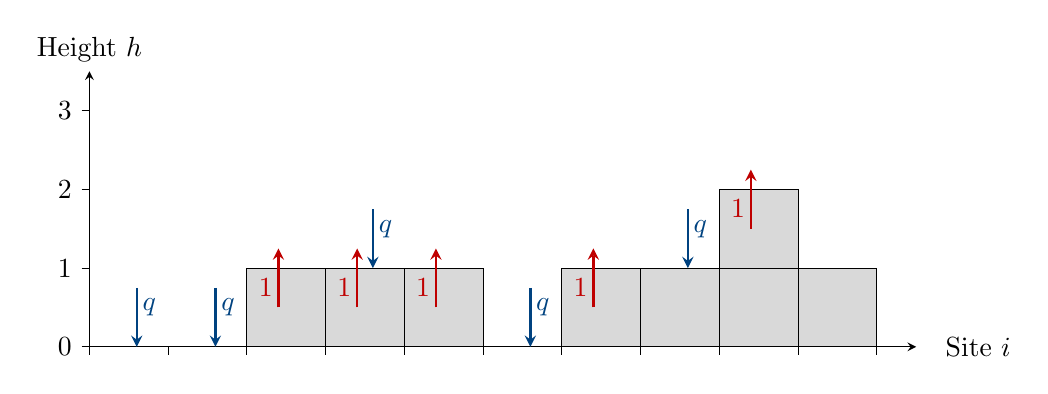
\begin{tikzpicture}

	% Coordinate system
	\newcommand\ticklength{0.1}
		% X
			\draw[->] (0,0) -- (10.5,0);
			\draw (10.75,0) node[anchor=west] {Site \(i\)};
			\foreach \x in {0,1,...,10} {
				\draw (\x, -\ticklength) -- (\x, 0);
			}
		% Y
			\draw[->] (0,0) -- (0,3.5);
			\draw (0,3.5) node[anchor=south] {Height \(h\)};
			\foreach \y in {0,1,...,3} {
				\draw (-\ticklength,\y) -- (0,\y);
				\draw (-\ticklength,\y) node[anchor=east] {\y};
			}

	% Boxes
		% Draws a box with the lower left corner at the specified coordinate
		\newcommand\drawbox[1] {
			\draw[fill=lgray] (#1) -- +(0,1) -- + (1,1) -- + (1,0) -- cycle;
		}
		\newcommand\evaporate[1] {
			\draw[->,thick,red] (#1) ++(0.4,0.5) -- +(0, 0.75);
			\draw[red] (#1) ++(0.45,0.75) node[anchor=east] {\(1\)};
		}
		\newcommand\deposit[1] {
			\draw[->,thick,blue] (#1) ++(0.6,0.75) -- +(0, -0.75);
			\draw[blue] (#1) ++(0.55,0.5) node[anchor=west] {\(q\)};
		}
		\drawbox{2,0}
		\drawbox{3,0}
		\drawbox{4,0}
		\drawbox{4,0}
		\drawbox{6,0}
		\drawbox{7,0}
		\drawbox{8,0}
		\drawbox{8,1}
		\drawbox{9,0}

		\evaporate{2,0}
		\evaporate{3,0}
		\evaporate{4,0}
		\evaporate{6,0}
		\evaporate{8,1}

		\deposit{0,0}
		\deposit{1,0}
		\deposit{3,1}
		\deposit{5,0}
		\deposit{7,1}
\end{tikzpicture}
	\caption[]{Illustration of a simple growth process. Particles are {\color{blue}deposited} and {\color{red}evaporated} at rates~{\color{blue}\(q\)} and~{\color{red}\(1\)}, respectively. However, an event is only allowed if the invariant that adjacent sites can only differ by a maximum of height~1 is maintained; as a result, only the transitions indicated by arrows are permitted.}
	\label{fig:growth process schema}
\end{figure}
%
For \(q_1 < 1\), it is known that the system behaves stationarily with an exponential probability distribution of the microstates,
%
\begin{equation}
	P(\{h_i\}) \propto q_1^{\sum_jh_j} = e^{-\mu_1 H}
\end{equation}
%
where \(\mu = -\ln q\) can be interpreted as a chemical potential and \(H = \sum_{i=1}^Nh_i\) is the total number of particles in the system. Comparing this with a Boltzmann distribution reveals that \(\mu\) plays the role of (inverse) temperature, and \(H\) is the energy contained in the system.

Making the connection to the previous section, a temperature quench manifests itself here as a ``deposition rate quench'', e.g. by changing said rate to another value \(q_2 < 1\) at \(t = \tau_0\), upon which the system will relax into a new equilibrium state. This is precisely what was previously done, and carrying over the analogy just mentioned in the last paragraph, this system should obey the fluctuation theorem
%
\begin{equation}
	\langle e^{\Delta\mu\Delta H}\rangle = 1
\end{equation}
%
where \(\Delta\mu = -(\ln q_2-\ln q_1)\) is what previously was an inverse temperature difference.

Figure~\RefFigure{fig:growth_process_plot} shows how the above average develops in simulations of small systems in a billion trials. Each experiment confirms the fluctuation theorem by clearly converging to \(1\).

Surprisingly, the quench over the phase transition into a nonequilibrium state (\(q_2 > 1\)) shows converging behaviour, which is something the theorem does not suggest, due to the assumption of having an equilibrium on either (far) end of the quenches. This suggests that the theorem could be more powerful than expected, and could e.g. be useful to find out properties of the critical point \(q = 1\) of the phase transition. At this point this remains entirely speculative though, and would be a suitable subject for further investigations.




\begin{figure}[htbp]
	\centering
	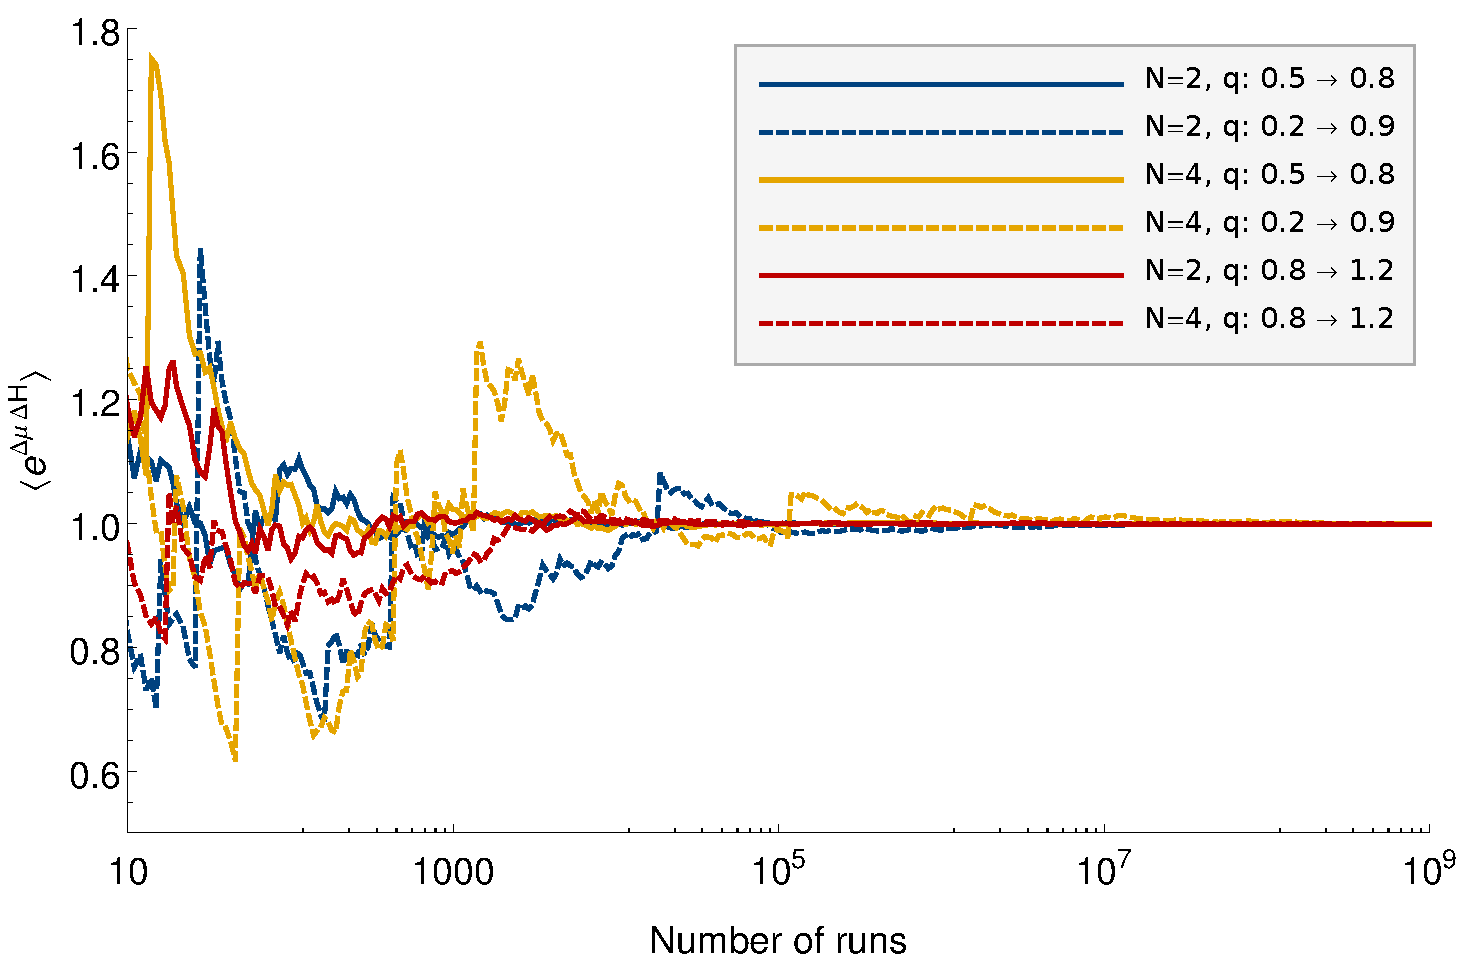
\includegraphics[width=30em]{figures/growth_process}
	\caption[]{Convergence of \(\langle e^{\Delta\mu\Delta H}\rangle\) to~1 in the growth model with system sizes of~{\color{blue}2} and~{\color{dyellow}4}. The initially empty lattice is equilibriated using 50 time steps to reach the initial configuration, before the final state is obtained using three additional steps. Each run records one value \(e^{\Delta\mu\Delta H}\), which is then averaged over many individual runs. The {\color{blue}blue} and {\color{dyellow}yellow} graphs show the development of said average over time in an ordinary quench, and confirm the fluctuation theorem's claim. The {\color{red}red} line corresponds to changing the rates so that the system is brought beyond the phase transition (\(q > 1\)); in this scenario, there is no relaxation into a new stationary state, as the interface grows arbitrarily high over time. Remarkably, the fluctuation theorem seems to hold even in this case, despite the assumption of asymptotic equilibrium in its derivation.}
	\label{fig:growth_process_plot}
\end{figure}




%%%%%%%%%%%%%%%%%%%%%%%%%%%%%%%%%%%%%%%%%%%%%%%%%%%%%%%%%%%%%%%%%%%%%%%%%%%%%%
\subsubsection{Nonequilibrium model on a small state space}
%%%%%%%%%%%%%%%%%%%%%%%%%%%%%%%%%%%%%%%%%%%%%%%%%%%%%%%%%%%%%%%%%%%%%%%%%%%%%%

To test the more general formula \RefEqn{eqn:SEnv fluctuation theorem}, namely
%
\begin{equation*}
	\tilde P(\Delta\SEnv = X) = e^X \tilde P(\Delta\SEnv = -X) ~,
\end{equation*}
%
a less specialized setup is necessary. Here, we will only assume the most basic requirements for this theorem, namely having a Markov process with time-independent rates; more explicitly, there will be no assumptions of equilibirum or asymptotic behaviour.

The system consists of a set of states \(c_i\in\Omega\) with \(|\Omega| = 8\), and therefore a transition matrix \(w_{c\to c'}\) with \(8^2-8 = 56\) nonzero entries (\(\forall c.\;w_{c\to c} = 0\)). Its elements are randomly chosen (strictly) between \(0\) and \(1\) before the experiment (and left fixed throughout each run). In a similar fashion, the initial distribution \(p^\init\) is determined.

A single run now consists of sampling an initial state from \(p^\init\), and letting it evolve in a Monte-Carlo simulation for some time \(T\) (here: \(1\)), corresponding to a certain amount of attempted state transitions (here: \(10^5\)). Each time the system's configuration changes, the generated \(\Delta\SEnv\) is recorded. As an additional consistency check, the overall distriburion of final states was checked against a numerical solution of the Mater equation
%
\begin{equation}
	\forall c.\;\dot p_c(t) = \underbrace{\sum_{c'}w_{c'\to c}p_{c'}(t)}_{\text{jump into } c} - \underbrace{\sum_{c'} w_{c\to c'}p_{c}(t)}_{\text{jump out of } c} ~,
\end{equation}
%
which describes the distribution of states on a statistical level directly, whereas the main simulation is based on individual runs, which are then later used for statistics.


A simulation now consists of a decent amount (\(10^7\)) individual runs, the result of which is then binned and put in a histogram. As can be seein in figures \RefFigure{fig:histogram_lin}~and~\RefFigure{fig:histogram_log}, the theorem is reproducible in simulation.


\begin{figure}[htbp]
	\centering
	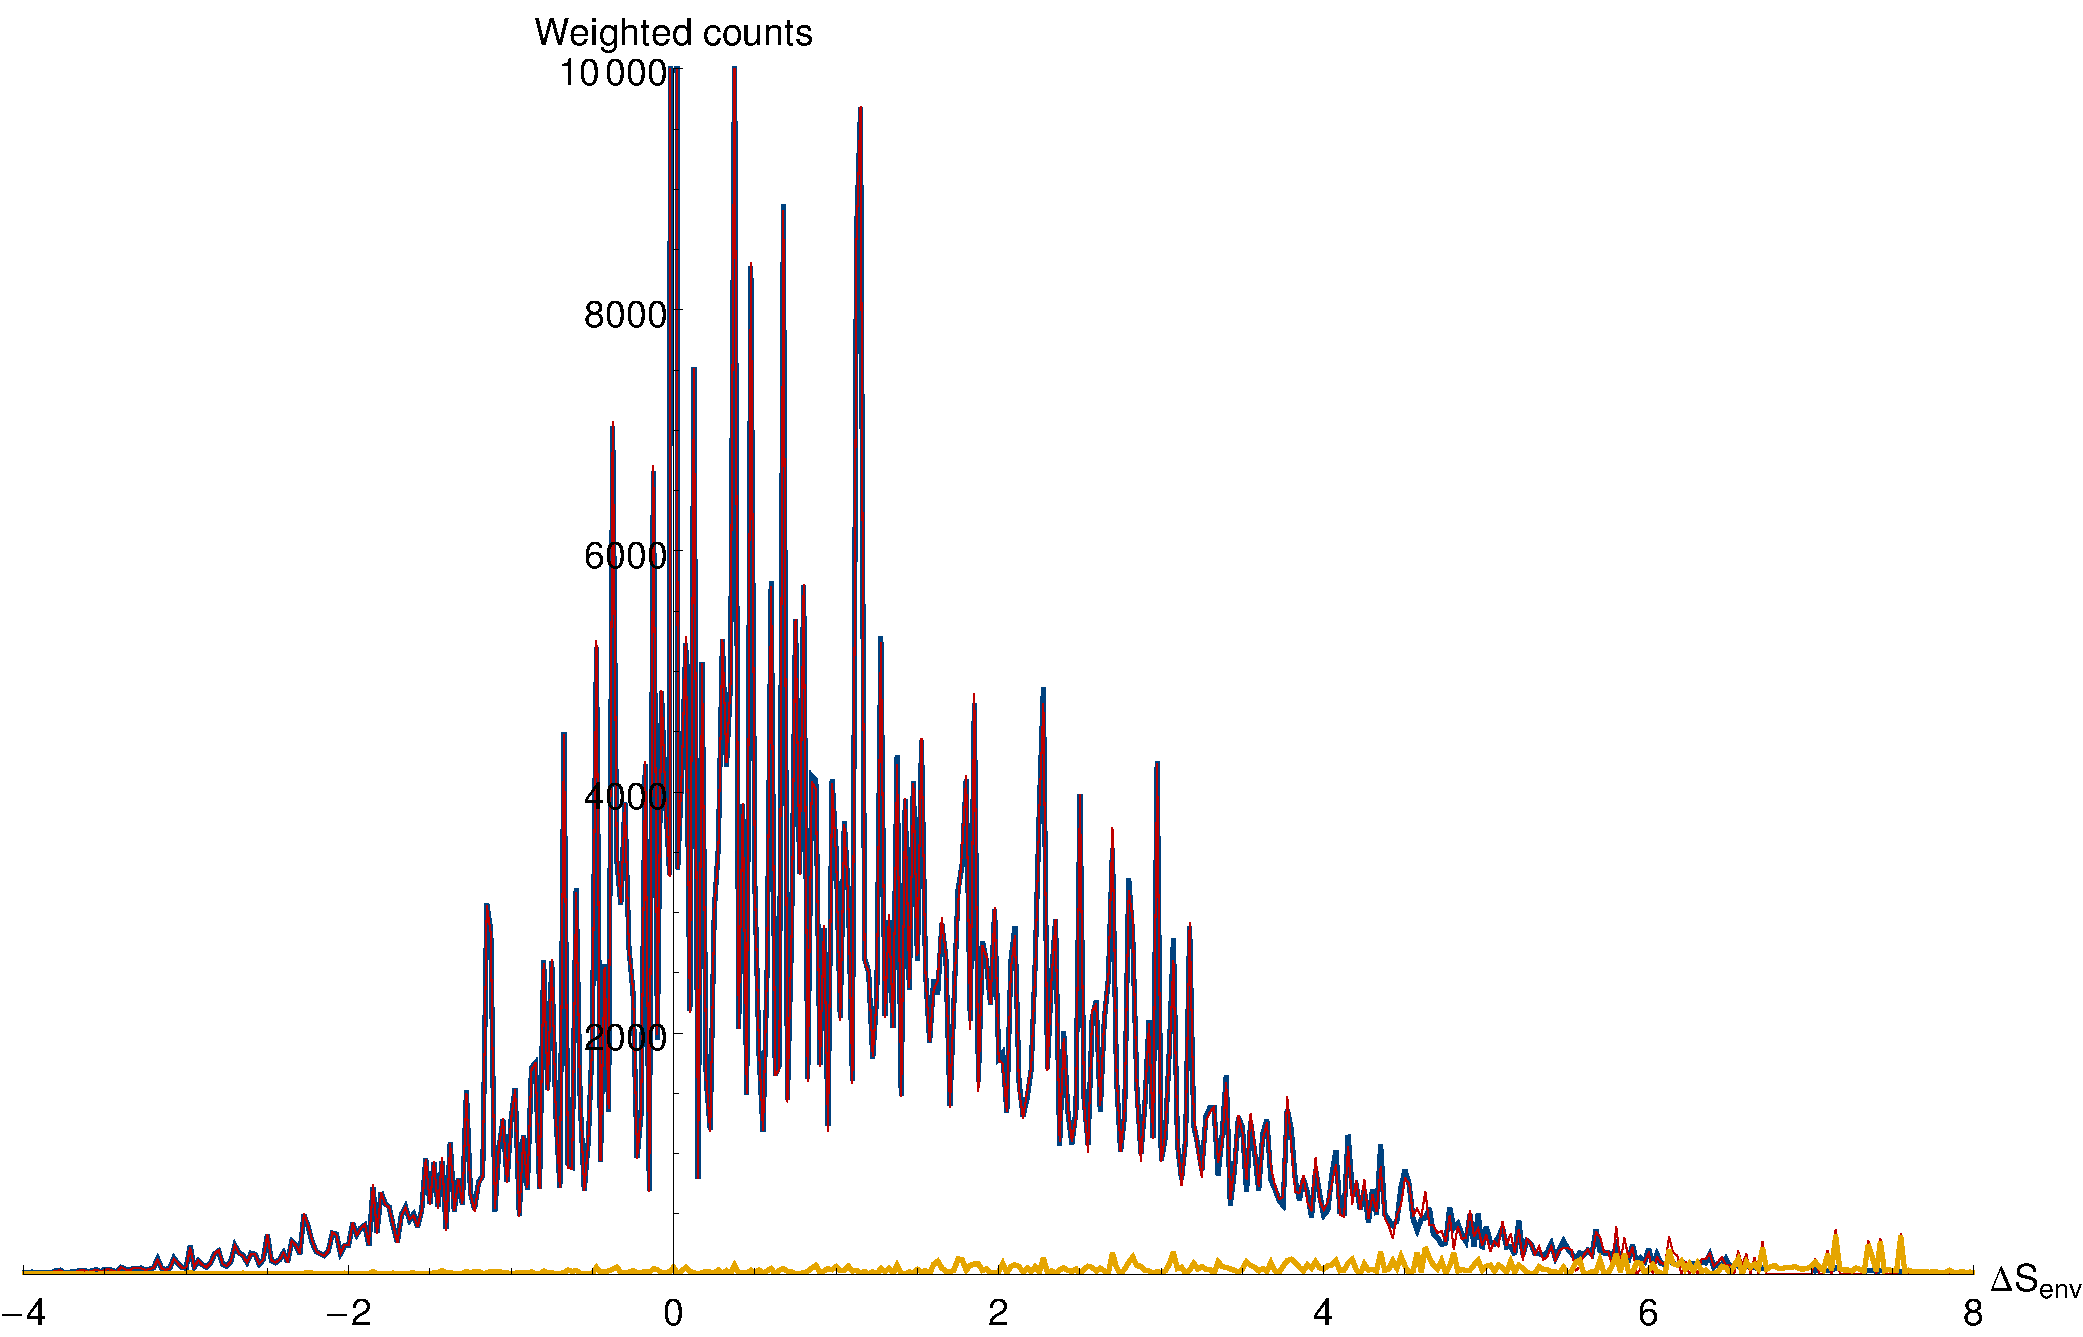
\includegraphics[width=30em]{figures/histogram_lin}
	\caption[]{Linear histogram of a simulation of the fluctuation theorem for \(\Delta\SEnv\), obtained by binning the results of \(10^7\) individual runs. Shown in {\color{blue}blue} and {\color{red}red} are the actual histogram and that histogram with the symmetry relation \(f(x) = e^xf(-x)\) (corresponding to the fluctuation theorem) applied; the {\color{dyellow}yellow} line is the (absolute) deviation between these two representations. It can be seen that both histograms match well, with only a few barely visible red peaks overshooting, which is visualized by the {\color{dyellow}yellow} graph more clearly. The overlap is especially good in the region around \(\Delta\SEnv = 0\) (most notably \emph{at} \(0\), where two peaks about \(5\cdot10^4\) meet), whereas in the large deviation regime towards the edges of the plot show rare events for which the statistics are not as good, but still well within acceptable bounds.}
	\label{fig:histogram_lin}
\end{figure}

\begin{figure}[htbp]
	\centering
	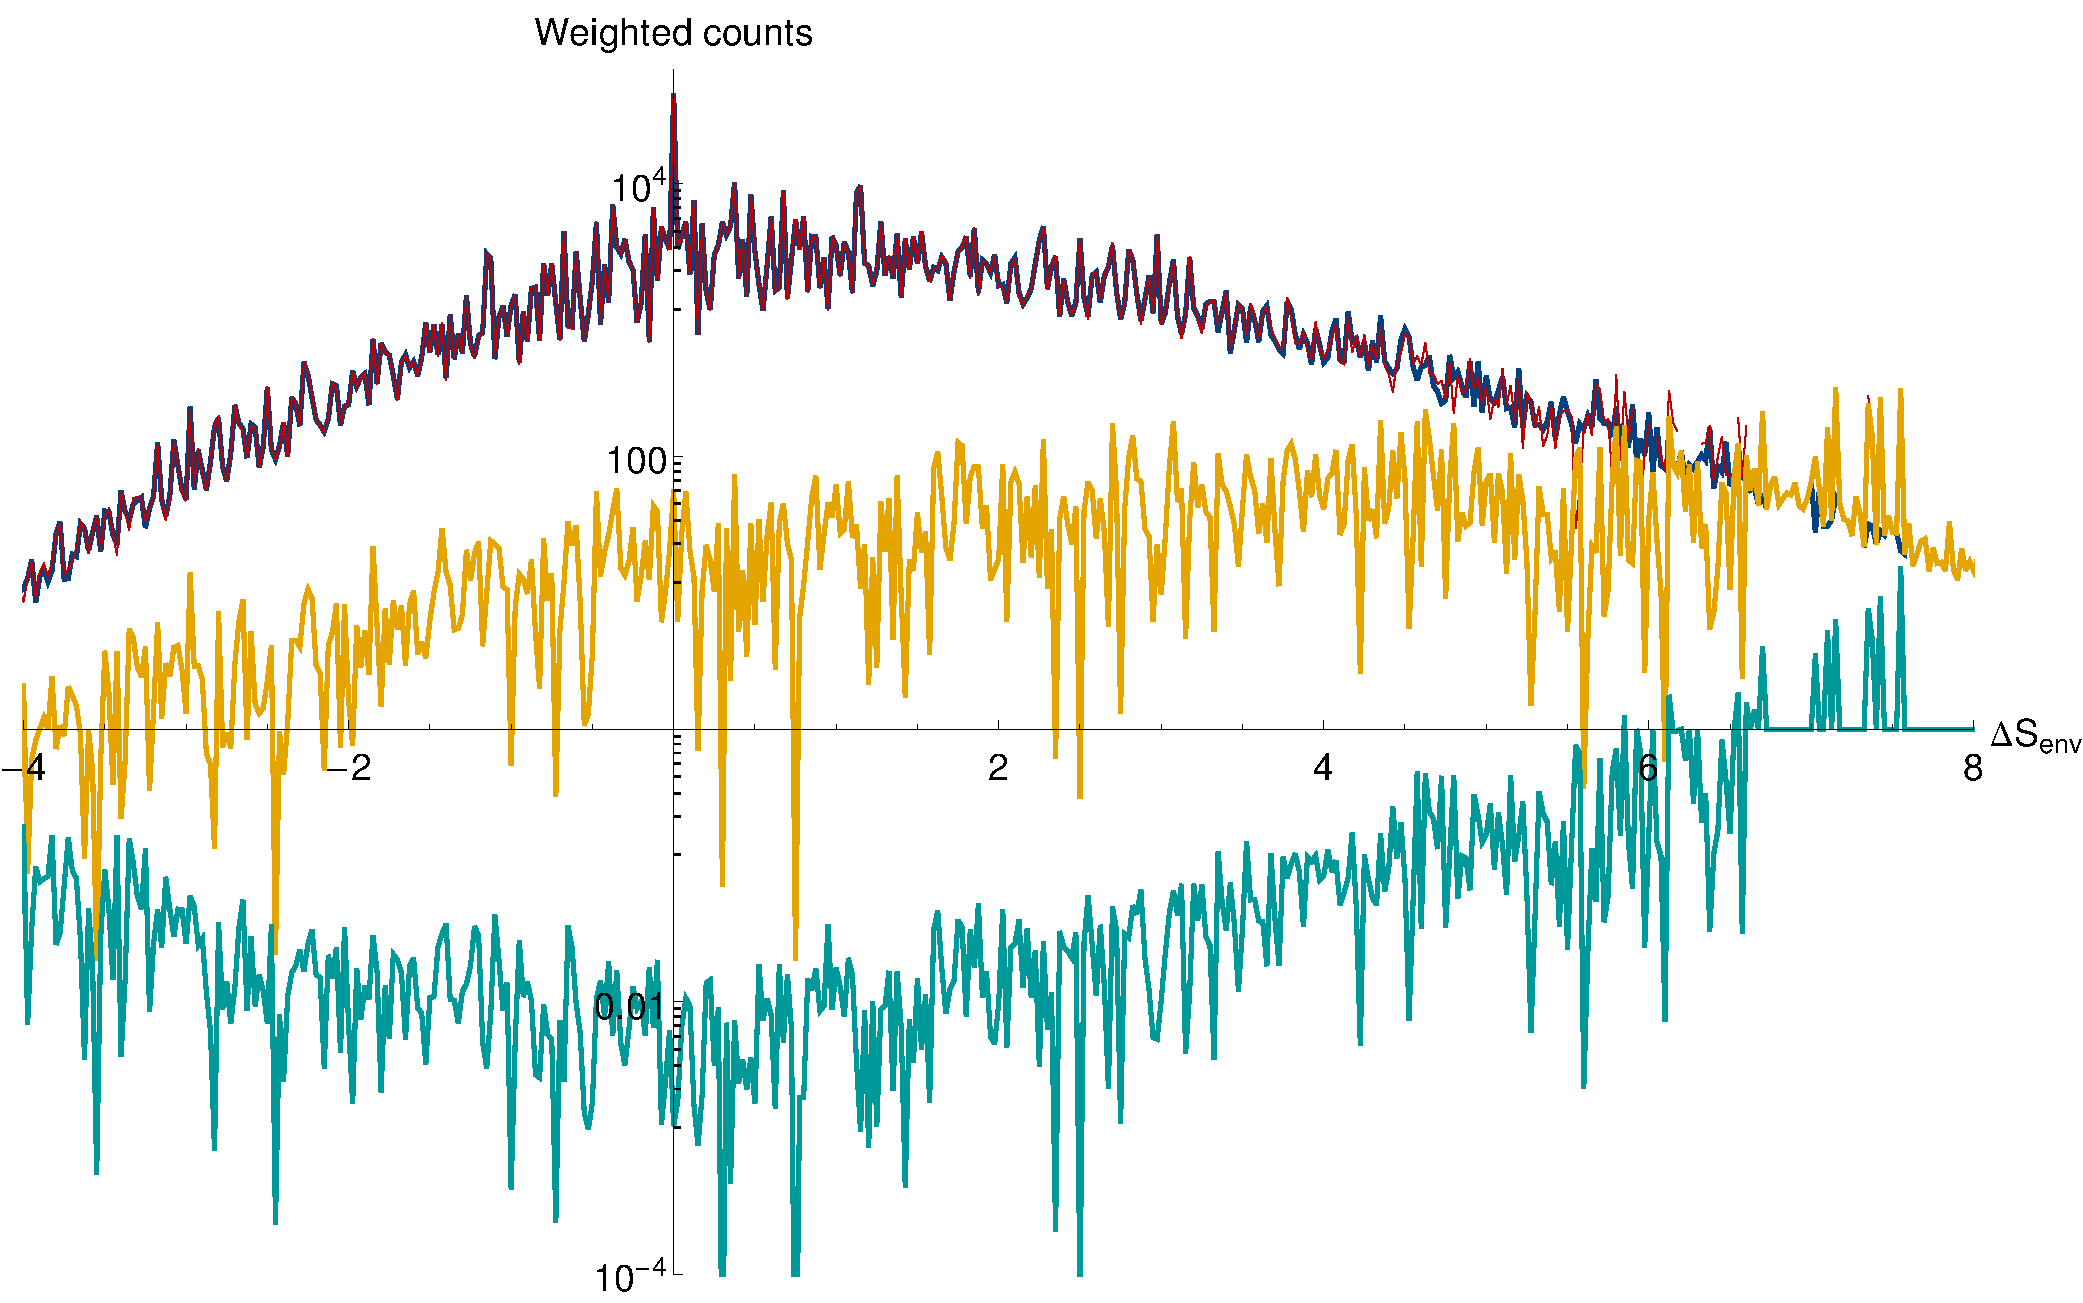
\includegraphics[width=30em]{figures/histogram_log}
	\caption[]{Same histogram as figure \RefFigure{fig:histogram_lin}, but with logarithmic \(y\)-axis. In addition to the graphs for the histogram ({\color{blue}blue}), the symmetrized version ({\color{red}red}, again just barely visible) and the absolute deviation ({\color{yellow}yellow}), this also shows the relative deviation in {\color{cyan}cyan}. This demonstrates again that both graphs match fairly well, particularly in around \(\Delta\SEnv = 0\), where most events happen. Leaving the middle region the overlap becomes worse as \(|\Delta\SEnv|\) increases, which can be explained by the fact that these events are relatively rare, hence the statistics aren't as good (compare e.g. about \(100\) weighted counts at \(\Delta\SEnv = 7\) vs. \(10^4\) around \(\Delta\SEnv = 1\)).}
	\label{fig:histogram_log}
\end{figure}

% Continuous phase space
\chapter{Entropy production in continuous phase space systems}
\label{chap:flow}

The contents of this chapter are again an in-depth description of a publication, this time in the Journal of Statistical Physics, under the same title \cite{flow-paper}.

An overview is as follows: The first section will talk about how to transfer some of the ideas used in the previous chapter to a continuous setting, and what problems arise on the way there. Afterwards, in section~\RefSection{sec:sde}, a brief overview over stochastic differential equations (SDEs) is given, before the main model of interest is introduced in section~\RefSection{sec:underdamped-model}. Section~\RefSection{sec:differential entropy production}, the chapter's main part, will then develop a new entropy definition, and compare it with a previously known one in the process.

The most important result will be that the production of environmental entropy is in a certain sense ambiguous, allowing multiple different definitions that all agree in their end results.


%%%%%%%%%%%%%%%%%%%%%%%%%%%%%%%%%%%%%%%%%%%%%%%%%%%%%%%%%%%%%%%%%%%%%%%%%%%%%%
\section{From discrete to continuous systems}
\label{sec:discrete to continuous}
%%%%%%%%%%%%%%%%%%%%%%%%%%%%%%%%%%%%%%%%%%%%%%%%%%%%%%%%%%%%%%%%%%%%%%%%%%%%%%

The basis of Chapter~\ref{chap:thingie} was the assumption of a discrete system \(\Omega = \{c_1, c_2, \ldots\}\). On the other hand, many processes occurring in nature are not discrete. This chapter describes an attempt to transfer the concept of environmental entropy used before to a continuous phase space system governed by Hamiltonian equations of motion.

Recall that a Markov process is fully described by an initial configuration \(p^\init\) and a set of transition rates \(w\), which provide a way of getting from one state to the next. Conceptually, this can be continualized to the case where the configuration is the location of a particle, leading to a system described by
%
\begin{equation}
	\label{eqn:overdamped}
	\dot q(t) = f(q,t) + g(q,t)\xi(t) ~,
\end{equation}
%
which can be understood in two different ways. Coming from a Markov process, \(f\) corresponds to the bias of the transition rates to go towards a certain state, and \(g\) accounts for how the noise depends on location. On the other hand, seen from a neutral standpoint, \(f\) is of course a force term, and \(g\xi\) is the randomness of the system due to a heat bath represented by Gaussian noise \(\xi(t)\), for example.

Most noticably, the above equation does not include any form of momentum. This can be seen as a residue of the Markov property, which was previously informally described as ``momentum-less''; in a continuous differential equation (DE), this description is much more meaningful, because very high damping gets rid of any momentum right away. For this reason, equations of the form \RefEqn{eqn:overdamped} are called \emph{overdamped}, and could for example describe the motion of a bacteria in water (which happens to be quite thick for small organisms \cite{sengupta}. Many of the quantities associated with Markov processes have clear corresponding quantities in the overdamped case, in particular the notion of a ``jump'' from one state to the other has a reverse, allowing the definition of environmental entropy to carry over quite directly \cite{seifert-overdamped},
%
\begin{equation}
	\Delta\SEnv = \ln\frac{p[\gamma | q_0]}{p^\dagger[\gamma^\dagger | q_0^\dagger]}
\end{equation}
%
where \(p[\gamma]\) is the probability of taking the forward path \(\gamma\), and \(p^\dagger[\gamma^\dagger]\) is the likelihood of walking that same path in reverse direction. The \(\dagger\) (``dagger'') or \emph{conjugation} operation encodes this reversal in the obvious way: for a process running from time \(t=0\) to \(T\),
%
\begin{equation}
	\begin{split}
		q^\dagger(t) &= q(T-t) \\
		q_0^\dagger(t) &= q_T \\
		t &\overset\dagger\rightarrow T-t
	\end{split}
\end{equation}
%
where the last line is important if the coefficients in \RefEqn{eqn:overdamped} have an explicit time dependency. Note that the \(\dagger\) operation is \emph{not reversing time}, it only stands for walking the same path in reverse directions, probably better described as ``making the same decisions, but in reverse order''. Figure~\RefFigure{fig:knight continuous} also illustrates this process.

\begin{figure}[htbp]
	\centering
	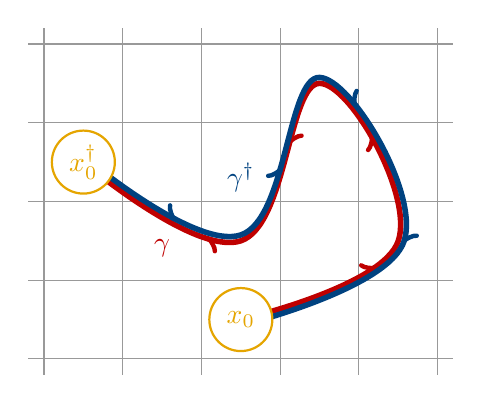
\begin{tikzpicture}[
		move1/.style={red, thick},
		move2/.style={blue, thick}
		]

	\draw[step=1cm, gray, shift={(0.5,0.5)}] (-3.2,-1.2) grid (2.2,3.2);


	\begin{scope}
		\newcommand\LineWidth{2}
		\draw[move1, line width=\LineWidth, postaction={decorate},
				decoration={
					markings,
					mark=at position .2 with {\arrow{left to};},
					mark=at position .4 with {\arrow{left to};},
					mark=at position .6 with {\arrow{left to};},
					mark=at position .8 with {\arrow{left to};}
				}
			]
			plot[smooth,tension=0.7] coordinates{(0,0) (2,1) (1,3) (0,1) (-2, 2)};
		\draw[move2, line width=\LineWidth, postaction={decorate},
				decoration={
					markings,
					mark=at position .25 with {\arrowreversed{right to};},
					mark=at position .45 with {\arrowreversed{right to};},
					mark=at position .65 with {\arrowreversed{right to};},
					mark=at position .85 with {\arrowreversed{right to};}
				}
			]
			plot[smooth,tension=0.7] coordinates{(0,0-0.075) (2+0.075,1) (1,3+0.075) (0,1+0.075) (-2, 2+0.075)};
	\end{scope}


	\newcommand\smallR{0.075}
	\newcommand\Move[3]{
		\draw[->, #3, shorten >= \smallR cm, shorten <= \smallR cm] #1 -- #2;
		\draw[#3] #2 circle (\smallR);
	}
	
	\node[move1] at (-1,0.9) { \(\gamma\) };
	\node[move2] at (0,1.8) { \(\gamma^\dagger\) };

	\draw[yellow, fill=white, thick] (-2,2) circle (0.4);
	\node[yellow] at (-2,2) { \(x_0^\dagger\) };

	\draw[color=yellow, fill=white, thick] (0,0) circle (0.4);
	\node[yellow] at (0,0) { \(x_0\) };

\end{tikzpicture}
	\caption[]{
		The knight from figure~\RefFigure{fig:knight}, but now in a continuous setting, where the configuration is \((x,y)\in\Set R^2\). The {\color{red}forward path \(\gamma\)} is taken with probability \(p[{\color{red}\gamma}|{\color{yellow}x_0}]\), and the {\color{blue}backward/conjugate path \(\gamma^\dagger\)} occurs with probability \(p^\dagger[{\color{blue}\gamma^\dagger}|{\color{yellow}x_0^\dagger}]\). In both cases, the paths can be constructed so time runs forward as the particle follows the trajectory.
	}
	\label{fig:knight continuous}
\end{figure}

Of course not all systems in nature are overdamped in the continuous case, just like not every discrete system has the Markov property. These non-overdamped -- \emph{underdamped} -- systems take the full Hamiltonian phase space into account, and the Hamiltonian equations of motion take the form
%
\begin{equation}\begin{split}
	\label{eqn:general hamiltonian equations}
	\dot q(t) &= f_q(q,p,t) + g_q(q,p,t)\xi_q(t) \\
	\dot p(t) &= f_p(q,p,t) + g_p(q,p,t)\xi_p(t)
\end{split}\end{equation}
%
As will be discussed later, it is nontrivial to introduce the concept of environmental entropy production in this scenario. The key reason to this is that a path cannot be reversed in a straight-forward way (i.e. the ``\(\dagger\)'' operation is not easily defined), and the main result of this chapter is a new way this path reversal can be defined, and what the consequences are.

To explain this, consider simply carrying over the \(\dagger\)~operation from the above (overdamped) case. The stochastic trajectory, now through \((q,p)\) space, will be transformed \`a la
%
\begin{equation}\begin{split}
	\gamma &= \Bigl\{\bigl(q(t),p(t)\bigr)\Bigr\}
	\\ \overset\dagger\longrightarrow \quad
	\gamma^{\dagger_\text{na\"ive}}
		&= \Bigl\{\bigl(q^{\dagger_\text{na\"ive}}(t),p^{\dagger_\text{na\"ive}}(t)\bigr)\Bigr\}
		= \Bigl\{\bigl(q(T-t),p(T-t)\bigr)\Bigr\}
\end{split}\end{equation}
%
but it turns out that the velocity \(\dot q\) has a different sign as momentum \(p\) in this definition, leading to an unphysical path.







%%%%%%%%%%%%%%%%%%%%%%%%%%%%%%%%%%%%%%%%%%%%%%%%%%%%%%%%%%%%%%%%%%%%%%%%%%%%%%
\section{Stochastic differential equations}
\label{sec:sde}
%%%%%%%%%%%%%%%%%%%%%%%%%%%%%%%%%%%%%%%%%%%%%%%%%%%%%%%%%%%%%%%%%%%%%%%%%%%%%%

There are multiple equivalent approaches to stochastic differential equations (SDEs), i.e. differential equations with a probabilistic or ``noise'' term. There are two important distinctions to make between the three commonly used ones.

The goal of this section is not providing an introduction to SDEs, but to illustrate different formalisms briefly, and mention their key concepts. A more rigorous yet practical treatment of stochastic calculus can be found in e.g. \cite{sde}, which also served as a main source for what follows.


%%%%%%%%%%%%%%%%%%%%%%%%%%%%%%%%%%%%%%%%%%%%%%%%%%%%%%%%%%%%%%%%%%%%%%%%%%%%%%
\subsection{Math vs. physics}
\label{sec:math vs physics}
%%%%%%%%%%%%%%%%%%%%%%%%%%%%%%%%%%%%%%%%%%%%%%%%%%%%%%%%%%%%%%%%%%%%%%%%%%%%%%

The area usually associated with stochastic differential equations in mathematics is \Ito{} calculus, while its close relative named after Stratonovich is what physics typically deals with. Both of these deal with equations of the form
%
\begin{equation}
	\label{eqn:sde}
	\d X_t = f(X_t,t) \d t + g(X_t,t) \d W_t
\end{equation}
%
describing how a \emph{microscopic} quantity \(X\) evolves under the influence of a deterministic drive \(f\) and a stochastic contribution \(g\,\d W_t\), where \(\d W_t\) is the Wiener measure accounting for the stochasticity. The Weiner process is the fundamental building block in SDEs; \(W_t\) can be interpreted as the position of a random walk at time \(t\), and \(\d W_t\) is a ``small'' increase of this random walk as time advances a little. The solution of such a SDE will be a probability distribution for the value of \(X\).
Informally -- but maybe more intuitive -- the above equation is ``divided by \(\d t\)'' to yield
%
\begin{equation}
	\dot X(t) = f(X(t),t) + g(X(t),t)\frac{\d W_t}{\d t} ~,
\end{equation}
%
called a Langevin equation, and \(\d W_t(t)/\d t\) can be interpreted as Gaussian noise \(\xi(t)\),
\begin{equation}
	\dot X(t) = f(X(t),t) + g(X(t),t)\xi(t)~.
\end{equation}
%
This is the form often used in physics. In this setting, the noise is usually defined by its statistical properties, most commonly
\begin{align}
	\langle\xi(t)\rangle &= 0 \\
	\langle\xi(t)\xi(t')\rangle &\propto \delta(t-t')
\end{align}
%
and can therefore be pictured as a quantity fluctuating around \(0\) so wildly that there are no correlations between any given different points in time. The advantage of this approach of course is that \(\xi\) can be treated as an ordinary function with certain special properties.


%%%%%%%%%%%%%%%%%%%%%%%%%%%%%%%%%%%%%%%%%%%%%%%%%%%%%%%%%%%%%%%%%%%%%%%%%%%%%%
\subsection{\Ito{} vs. Stratonovich}
\label{sec:ito-stratonovich dilemma}
%%%%%%%%%%%%%%%%%%%%%%%%%%%%%%%%%%%%%%%%%%%%%%%%%%%%%%%%%%%%%%%%%%%%%%%%%%%%%%

There is a surprising difference between the \Ito{} and Stratonovich schemata used to describe a system's behaviour. Suppose one wanted to solve a SDE numerically. The naive approach would take the current state of the system \(X(t)\), and extrapolate its new value using the SDE (using a suitably generated random number \(\Cal R\) for the noise) a timespan \(\d t\) later \`a la
%
\begin{equation}
	X(t+\d t) = f(X(t))\d t + g(X(t)) \Cal R ~.
\end{equation}
%
However, this leaves one question open: why should the functions be evaluated at the starting point of the interval \([t,t+\d t]\), and not for example at \(t_\text{eval} = t+\d t/2\)? And indeed it turns out that the result depends on the choice of this evaluation point. In other words, there is an ambiguity in solving SDEs: all of the schemata
%
\begin{align}
	X(t+\d t) &= f(X(t+a\,\d t))\d t + g(X(t+a\,\d t)) \Cal R \\
	a &\in [0,1]
\end{align}
%
are theoretically valid ways of defining the integration of \RefEqn{eqn:sde}. Which value of \(a\) to choose depends on a number of factors, a couple of which are:
%
\begin{itemize}
	\item \emph{Modelling.} What is the nature of the noise? In finance, the randomness of the market is assumed to be a result of the current state and appears random due to the fact people are unpredictable. This is what the \Ito{} method models by setting \(a = 0\). On the other hand, for example in physics or biology, the noise often originates from a second, underlying and inaccessible process, such as temperature-related fluctuations, and setting \(a = 1/2\) (=~Stratonovich) accounts for this independence of noise and system by not preferring either side of the timestep over the other. Other values of \(a\) are not commonly used, although they do appear in special cases \TODO{ref: jaegon mentioned \(a=1\)}.
	\item \emph{Pragmatism.} Some formulas are easier in certain formulations. A good example is the chain rule, which is called just that in the Stratonovich case, whereas its analogon has the telling name ``\Ito{}'s lemma''.
\end{itemize}
%
In the context of these issues, it is important to mention that both approaches are equvalent and can be converted into each other via
%
\begin{equation}
	\int_0^Tf(W_t,t)\circ\d W_t
	=
	\int_0^Tf(W_t,t)\,\d W_t
	+
	\frac12\int_0^T \partial_xf(W_t,t)\,\d t ~,
\end{equation}
%
where the convention is that ``\(\circ\,\d W_t\)'' stands for Stratonovich integration, and anything without special syntax is \Ito{}. The spatial derivative \(\partial_x\) is to be read as with respect to \(f\)'s first argument (which appears with explicit mention of the Wiener process in the integrands). As can be seen above, both approaches are identical if the integrand \(f\) is spatially constant; otherwise, the nonvanishing integral will be referred to as a \emph{drift term}.


%%%%%%%%%%%%%%%%%%%%%%%%%%%%%%%%%%%%%%%%%%%%%%%%%%%%%%%%%%%%%%%%%%%%%%%%%%%%%%
\subsection{Micro vs. macro}
\label{sec:fp introduction}
%%%%%%%%%%%%%%%%%%%%%%%%%%%%%%%%%%%%%%%%%%%%%%%%%%%%%%%%%%%%%%%%%%%%%%%%%%%%%%

SDEs like eq.~\RefEqn{eqn:sde} assume a single quantity \(X\), tracks its behaviour over time, and accumulates this in a final probability distribution for its value. This is a microscopic approach, effectively equivalent to repeating the same experiment with identical initial conditions (i.e. particle in the same place) many times, recording each individual result, and putting that in a histogram.

However, individual partcles are rarely\footnote{For a case where this \emph{is} possible, consider biophysical models of individual cells, or the Brownian motion of small particles in liquid \cite{sengupta}.} accessible, and the starting point of the experiment is a probability distribution in the first place. This scenario is described by the Fokker-Planck (FP) equation, which can be interpreted as a generalized Heat Equation:
%
\begin{equation}
	\label{eqn:fp}
	\begin{split}
	\partial_tP(x,t)
	&= - \partial_x (f(x,t)P(x,t)) + \partial_x^2 (D(x,t)P(x,t)) \\
	&= -\partial_xj(x,t)
	\end{split}
\end{equation}
%
Like the Heat Equation, the FP equation describes a flow in terms of a current, just that this current can be more complex. Nevertheless, it still describes the evolution of an entire distribution over time, and not of one of its constituents. It can be shown that the FP equation is an alternative and equivalent formulation of the SDE
%
\begin{align}
	\d X_t = f(X_t,t)\d t + \sqrt{2 D(X_t,t)}\,\d W_t ~.
\end{align}
%
when integrated according to the \Ito{} calculus \cite{sde}.




%%%%%%%%%%%%%%%%%%%%%%%%%%%%%%%%%%%%%%%%%%%%%%%%%%%%%%%%%%%%%%%%%%%%%%%%%%%%%%
\section{Underdamped particle with additive noise}
\label{sec:underdamped-model}
%%%%%%%%%%%%%%%%%%%%%%%%%%%%%%%%%%%%%%%%%%%%%%%%%%%%%%%%%%%%%%%%%%%%%%%%%%%%%%

The treatment of the most general case of Hamiltonian motion, as stated for a single particle in \RefEqn{eqn:general hamiltonian equations}, turns out to be very complicated. For this reason, the model used here is a special case of said equations. That is not to say it is impractical though; many of the basic systems of classical mechanics can be described by these equations:
%
\begin{equation}\boxed{\begin{split}
	\label{eqn:model hamiltonian eqns of motion}
	\dot q &= p \\
	\dot p &= -V'(q) - \mu(p)p + \Gamma(p)\xi(t)
\end{split}}\end{equation}
%
This models a single one-dimentional particle of unit mass in full phase space \((q,p)\) subject to a conservative force field \(-V'(q)\), momentum-dependent friction \(\mu(p)\) and multiplicative noise \(\Gamma(p)\xi(t)\), where \(\xi(t)\) is Gaussian noise, implicitly defined via
%
\begin{equation}\begin{split}
	\langle\xi(t)\rangle &= 0 \\
	\langle\xi(t)\xi(t')\rangle &= 2D\delta(t-t')
\end{split}\end{equation}
%
and \(D\) is a diffusive coefficient.

The main question this chapter is trying to answer is what mechanism leads to the production of environmental entropy in a system that follows the above dynamics. In the sense of classical thermodynamics, environmental entropy can be thought of as the flow of energy in the form of heat in and out of a system (held at constant temperature). In the specific case here, the noise \(\xi\) adds energy to the system (decreasing the entropy in the environment due to the resulting cooling), while the friction takes out heat (increasing the entropy in the environment). Equipped with this simple knowledge of classical thermodynamics, it is already possible to formulate a definition for environmental entropy for a special case of the present model, namely if the particle is in equilibrium with a heat bath of temperature \(T\),
%
\begin{equation} T\d\SEnv = -\d Q \end{equation}
%
where \(Q\) is the heat contained in the system, and \(\SEnv\) is the environment's entropy. Since heat flowing from the environment into the system increases its entropy by \(\d\SEnv\) while decreasing the heat of the environment by \(\d Q\), a negative sign appears in the equation. Due to conservation of energy (first law of thermodynamics in the absence of mechanical work), the heat flow is precisely the energy flow between the systems, \(\d Q = \d E\), and \(E\) is simply the particle's energy,
%
\begin{equation} E = \frac{p^2}2 + V(q) \end{equation}
%
allowing the entropy production \(\d\SEnv\) to be written as
%
\begin{align}
	\d\SEnv(q,p) &= -\beta\,\d\left(\frac{p^2}2 + V(q)\right) \notag \\
	\Rightarrow \d\SEnv(q,p) &= -\beta p\d p - \beta V'(q)\d q ~.
	\label{eqn:classical environmental entropy production}
\end{align}
%
Reproducing this result from a microscopic approach however is nontrivial, and poses a strong consistency check for any theory trying to explain environmental entropy production in a similar setting. It will later turn out that under certain circumstances, some \emph{correct} theories fail to do so, yet yield correct physical results after another calculation. The reason and significance of this will be discussed at that point, where the terminology and formalism to deal with location-dependent ``thermodynamic'' quantities, like \(\d\SEnv(q,p)\) above, has been developed.






%%%%%%%%%%%%%%%%%%%%%%%%%%%%%%%%%%%%%%%%%%%%%%%%%%%%%%%%%%%%%%%%%%%%%%%%%%%%%%
\subsection{Fokker-Planck equation}
%%%%%%%%%%%%%%%%%%%%%%%%%%%%%%%%%%%%%%%%%%%%%%%%%%%%%%%%%%%%%%%%%%%%%%%%%%%%%%

A key quantity later will be the propagator of the Fokker-Planck equation, which can be seen as the continuous analogon of the Master quation \RefEqn{eqn:master}. For this reason, \RefEqn{eqn:model hamiltonian eqns of motion} has to be transformed into Fokker-Planck form. This will be done following the notation of \cite{sf} and defining phase space coordinates \(\vec x = (q,p)\), allowing it to be written as
%
\begin{equation}
	\d x_i = A_i(\vec x,t)\d t + B_i(\vec x, t)\d W_i
\end{equation}
%
where, as introduced in section~\ref{sec:math vs physics}, \(\d W_i\) can be interpreted as the random walk generated by the noise \(\xi(t)\).

The FP equation introduced in \ref{sec:fp introduction} was just concerned with a single dimension. In the present two-dimensional space (with coordinates \(\vec x\)), that equation has to be modified to
%
\begin{align}
	\label{eqn:fp phase}
	\partial_tP(\vec x,t)
	&= - \sum_{i=q,p} \partial_{x_i} (f_i(\vec x,t)P(\vec x,t)) + \partial_{x_i}^2 (D_i(\vec x,t)P(\vec x,t)) \\
	&= - \sum_{i=q,p} \partial_{x_i}j_i(\vec x,t)
\end{align}
%
taking into account the individual fluctuations each component of \(\vec x\) may be subject to. The coefficients are related to the above Langevin equation via
%
\begin{align}
	f_i(\vec x,t) &= A_i(\vec x,t) \\
	D_i(\vec x,t) &= \frac12B_i(\vec x,t)^2
\end{align}
%
when integrating accoring to \Ito{} scheme, done so for pragmatic reasons (there will be plenty of probably more interesting ambiguities later).
The FP equation corresponding to \RefEqn{eqn:model hamiltonian eqns of motion} there turns out to be
%
\begin{equation}\begin{split}
	\partial_t P(q,p,t) &= \Cal L \, P(q,p,t) \\
	\Cal L &= \mu(p)+p\mu'(p) + \Gamma(p)\Gamma''(p) + \Gamma'(p)^2 \\
	&\qquad +\bigl(p\mu(p) + 2\Gamma(p)\Gamma'(p) + V'(q)\bigr)\partial_p \\
	&\qquad +\frac12\Gamma(p)^2\partial_p^2 - p\partial_q ~.
\end{split}\end{equation}






%%%%%%%%%%%%%%%%%%%%%%%%%%%%%%%%%%%%%%%%%%%%%%%%%%%%%%%%%%%%%%%%%%%%%%%%%%%%%%
\subsection{Detailed balance redux}
%%%%%%%%%%%%%%%%%%%%%%%%%%%%%%%%%%%%%%%%%%%%%%%%%%%%%%%%%%%%%%%%%%%%%%%%%%%%%%

The idea of detailed balance (section \RefSection{sec:detailed balance}) is also applicable to continuous system, where as mentioned the Fokker-Planck equation \RefEqn{eqn:fp} takes over for the Master equation \RefEqn{eqn:master}. Analogous, a stationary FP equation means all macroscopic state variables are constant; in the present context it is of particular interest that no heat or environmental entropy is exchanged with the bath.

This can probably be better understood than in the discrete scenario even, where the explanation was quite abstract (``probability currents cancel out''). Eqns. \RefEqn{eqn:model hamiltonian eqns of motion} contains a friction term responsible for heating up the environment as the system moves, and also a noise term transferring energy (also in the form of heat) into the system. If these two contributions cancel out just right, then all that's left is a Hamiltonian system of a free particle in a potential, which is of course reversible and does not produce any heat.

Being in detailed balance introduces a connection between the friction terms \(\mu(p)\) and the noise coefficient \(\Gamma(p)\) in \RefEqn{eqn:model hamiltonian eqns of motion}. This relation can be obtainex explicitly by inserting a Boltzmann distribution (which is the equilibrium distribution of a system in thermal equilibrium with a heat bath) into the FP equation \RefEqn{eqn:fp phase} and setting it equal zero, namely
%
\begin{equation}
	P_\text{Boltz}(q,p)
	= \frac1Ze^{-\beta E(q,p)}
	= \frac1Z\exp\Bigl(-\beta \bigl(\tfrac{p^2}2+V(q)\bigr)\Bigr)
\end{equation}
%
The result is a first-order differential equation for \(\mu(p\)),
%
\begin{equation}\begin{split}
	0
	&=
	\frac12 \beta^2 p^2 \Gamma(p)^2
	- \beta p^2 \mu(p)
	- 2 \beta p \Gamma(p) \Gamma'(p)
	- \frac12 \beta  \Gamma(p)^2
	\\&\qquad
	+\Gamma(p) \Gamma''(p)
	+ \Gamma'(p)^2
	+ p \mu'(p)
	+ \mu(p)  ~.
\end{split}\end{equation}
%
Thanks to computer algebra systems\footnote{Mathematica~9.0.0.0}, the solution of this daunting equation is obtained quite easily, it is
%
\begin{equation}
	\mu(p) = \frac12\beta\Gamma(p)^2 - \frac1p\Gamma(p)\Gamma'(p) + C\frac1pe^{\frac{\beta p^2}2}
\end{equation}
%
where \(C\) is an arbitrary integration constant. However, since the last term is exponentially divergent for \(p\to\infty\), it unphysical: the mean acceleration of a system in equilibrium would be infinite. Therefore \(C = 0\) is the only suitable choice, and what remains is
%
\begin{equation}
	\label{eqn:einstein}
	\mu(p) = \frac12\beta\Gamma(p)^2 - \frac1p\Gamma(p)\Gamma'(p) ~.
\end{equation}
%
This generalizes the usual condition for detailed balance \(\mu = \frac12\beta\Gamma^2\) (also known as the Einstein relation) for momenum-independent (``additive'') noise and linear friction.



%%%%%%%%%%%%%%%%%%%%%%%%%%%%%%%%%%%%%%%%%%%%%%%%%%%%%%%%%%%%%%%%%%%%%%%%%%%%%%
\subsection{Short-time propagator}
%%%%%%%%%%%%%%%%%%%%%%%%%%%%%%%%%%%%%%%%%%%%%%%%%%%%%%%%%%%%%%%%%%%%%%%%%%%%%%

\subsubsection{General case}
\label{sec:general propagator case}

Like in the discrete case, a key ingredient to defining entropy production in a continuous setting is the notion of a path probability. This probability is given by the propagator or Green's function of the FP equation. It will be denoted \(G(\vec x'|\vec x;\,\Delta t)\), and can be read as the probability that a particle starting at phase space coordinates \(\vec x = (q,p)\) is found at a new point \(\vec x' = (q',p')\) at \(\Delta t\) time later. In the present work however, it will be sufficient to take the \emph{short-time} proagator into account, i.e. \(\Delta t\) is very small.

The short-time propagator \(G(\vec x'|\vec x;\,\d t)\) solves the FP equation to leading order in \(\d t\), and is therefore not uniquely defined:
%
\begin{enumerate}
	\item The short-time propagator need not be Gaussian, as long as the (``arbitrary-time'') macroscopic propagator is reproduced by it. According to the central limit theorem, any distribution with the correct first and second moments is sufficient. (Intuitively, this can be understood by the fact that many functions have identical first-order power series coefficients, but their actual global shape is influenced by the higher-order terms. In the present scenario, these terms are neglected, leading to said ambiguity.)
	%
	\item It is not clear where the fields contained in the FP equation \RefEqn{eqn:fp phase}, \(f_i(\vec x,t)\) and \(D_i(\vec x,t)\), have to be evaluated: at \(\vec x\), \(\vec x'\), between, somewhere in the neighbourhood? In general, an evaluation point at any \(\vec r = \varphi(\vec x,\vec x')\) with bijective \(\varphi\) will do \cite{wissel}. Conceptually, this is similar to the \Ito{}-Stratonovich dilemma introduced in the conext of stochastic differential equations in section~\RefSection{sec:ito-stratonovich dilemma}, but it is important to emphasize that this is a \emph{new, independent} ambiguity in addition to the previous one (which was resolved to integration according to \Ito{} scheme to obtain the FP equation from the SDE).
\end{enumerate}
%
To get a hold of the infinitely many short-time propagators, assume the evaluation point is linearly between the two end points,
%
\begin{equation}
	\vec r = (1-a)\vec x + a\vec x' \qquad a\in[0,1] ~,
\end{equation}
%
as done in \cite{sf}. Using \cite{wissel, donoso} this leads to the following expression for the propagator:
%
\begin{equation}\begin{split}
	\label{eqn:propagator general}
	G_a(\vec x'|\vec x;\,\d t)
	&= \prod_i \frac1{\sqrt{2\pi D_i\d t}}
	\\&\qquad
	\exp\left(
		- \frac{(\d x_i-A_i\d t+2aD_i'\d t)^2}{4D_i\d t}
		- a A_i'\d t
		+ a^2 D_i''\d t
		\right)
\end{split}\end{equation}
%
with the short-hands
%
\begin{align*}
	A_i &= A_i(\vec r,t)  &  A_i' &= \partial_{r_i}A_i(\vec r,t) \\
	D_i &= D_i(\vec r,t)  &  D_i' &= \partial_{r_i}D_i(\vec r,t)  &  D_i'' &= \partial_{r_i}^2D_i(\vec r,t) ~.
\end{align*}


\subsubsection{Applied to the model}

The system in question, \RefEqn{eqn:model hamiltonian eqns of motion}, consists of two coupled differential equations, but only one of them is stochastic, giving \(D_1\equiv0\). However, the propagator \RefEqn{eqn:propagator general} requires dividing by this quantity so it is not well-defined. For this reason, \RefEqn{eqn:model hamiltonian eqns of motion} is modified to add a ``very small'' (new, independent from \(\xi_p\)) noise term to the location, resulting in the system
%
\begin{equation}
	\label{eqn:underdamped sde epsilon}
	\begin{split}
		\dot q(t) &= p + \varepsilon \xi_q(t) \\
		\dot p(t) &= -V'(q) - \mu(p)p + \Gamma(p)\xi_p(t) ~;
	\end{split}
\end{equation}
%
the coefficient \(\varepsilon\) will later fall away on its own, justifying this rather ad-hoc addition.
The resulting propagator for this model then reads \TODO{check for correctness}
%
\begin{equation}
	\label{eqn:short time propagator}
	\begin{split}
		_\varepsilon G_a (q',p' | q,p;\,\d t)
		&= \frac1{2\pi\varepsilon\Gamma(r)\d t}
			\exp\Bigl(
				a^2(\Gamma(r)\Gamma''(r) + \Gamma'(r)^2)\d t
			\\&\quad
			-\frac{\bigl(V'(q+a\,\d q)\d t + 2 a\Gamma(r)\Gamma'(r)\d t + \d p + r\mu(r)\d t\bigr)^2}{2\Gamma(r)^2\d t}
			\\&\quad
			+ a\bigl(r\mu'(r)+\mu(r)\bigr)\d t
			- \frac{(\d q - r\d t)^2}{2\varepsilon^2\d t}
			\Bigr)
	\end{split}
\end{equation}
%
with
\begin{align*}
	\d q &= q' - q  &  \d p &= p' - p  &  r &= (1-a)p + ap' ~.
\end{align*}

As a consistency check, consider the limit \(\varepsilon\to0\). According to the differential equations above, this system should be deterministic in the position coordinate. And indeed the terms involving \(\varepsilon\) in \RefEqn{eqn:short time propagator} are of Gaussian shape, just like in the usual derivation of the \(\delta\)~distribution from a narrow Gaussian. More explicitly, the limit reads
%
\begin{equation}
	\label{eqn:delta-limit}
	\begin{split}
		G_a (q',p' | q,p;\,\d t) =
		\frac{\delta(\d q-r\d t)}{\sqrt{2\pi\d t}\Gamma(r)}\exp(\cdots)
	\end{split}
\end{equation}
%
where the \(\delta\) accounts for the deterministic location.



%%%%%%%%%%%%%%%%%%%%%%%%%%%%%%%%%%%%%%%%%%%%%%%%%%%%%%%%%%%%%%%%%%%%%%%%%%%%%%
\section{Differential entropy production}
\label{sec:differential entropy production}
%%%%%%%%%%%%%%%%%%%%%%%%%%%%%%%%%%%%%%%%%%%%%%%%%%%%%%%%%%%%%%%%%%%%%%%%%%%%%%

The focus of the main part of this chapter is the definition of differential environmental entropy \(\d\SEnv\). The term \emph{differential} will be used in multiple similar but different contexts; it can always be understood as some form of Taylor expansion of the finite entropy increase \(\Delta\SEnv\) in \(\d t\), \(\d q\) and \(\d p\) to lowest order. Which meaning is appropriate will be specified explicitly in ambiguous places.

The outline of what follows is this. First, an overview of Spinney and Ford's approach to defining \(\d\SEnv\) is given, which leads to the question what should be ``the state'' of an SDE. Inspired by this question, a new way of defining \(\d\SEnv\) will be proposed, and frequently compared to the other approach in the process of finding the corresponding formulas.



%%%%%%%%%%%%%%%%%%%%%%%%%%%%%%%%%%%%%%%%%%%%%%%%%%%%%%%%%%%%%%%%%%%%%%%%%%%%%%
\subsection{Spinney and Ford's entropy definition}
%%%%%%%%%%%%%%%%%%%%%%%%%%%%%%%%%%%%%%%%%%%%%%%%%%%%%%%%%%%%%%%%%%%%%%%%%%%%%%


In order to solve the issue of na\"ive path reversal mentioned in section~\RefSection{sec:discrete to continuous}, Spinney and Ford (SF) \cite{sf} choose to reverse time itself (\(t\to-t\)); more precisely, they take the time parity of all quantities into account, and mirror only those changing sign under time reversal. More explicitly, what they do is defining \(\dagger\) as \cite{sf-odd-even}
%
\begin{equation}\begin{split}
	\gamma &= \Bigl\{\bigl(q(t),p(t)\bigr)\Bigr\}
	\\ \overset\dagger\longrightarrow \quad
	\gamma^{\dagger_\SF}
		&= \Bigl\{\bigl(q^{\dagger_\SF}(t),p^{\dagger_\SF}(t)\bigr)\Bigr\}
		= \Bigl\{\bigl(\varepsilon q(T-t),\varepsilon p(T-t)\bigr)\Bigr\}
\end{split}\end{equation}
%
where \(\varepsilon\) is a parity operator, and equates to \(+1\) for even quantities such as \(q\) and \(-1\) for odd ones such as \(p\) under time reversal. Using this, they are able to use the entropy definition
%
\begin{equation}
	\Delta\SEnv = \ln\frac{p[\gamma | q_0]}{p^{\dagger_\SF}[\gamma^{\dagger_\SF} | q_0^{\dagger_\SF}]}
\end{equation}
%
to derive an expression for the differential environmental entropy production of arbitrary underdamped stochastic systems in full phase space \cite{sf}, given by
%
\begin{equation}
	\d\SEnv^\SF = \ln \frac{G_a(\vec x'|x;\,\d t)}{G_b(\vec x'^\dagger|\vec x^\dagger;\,\d t)} ~;
\end{equation}
%
recall that the propagator \(G_a(\vec x'|x;\,\d t)\) acorresponds to the probability to go from \(\vec x = (q,p)\) to \(\vec x'\) in the short time \(\d t\), plus an ambiguity parameter \(a\). In the case of the underdamped particle \RefEqn{eqn:underdamped sde epsilon} this then reads
%
\begin{equation}
	\label{eqn:DSEnv spinney main definition}
	\d\SEnv^\SF =
		\ln \frac
			{_\varepsilon G_a(q',p'|q,p;\,\d t)}
			{_\varepsilon G_b(q,-p|q',-p';\,\d t)} ~.
\end{equation}
%
A graphical representation of the paths constructed here can be found in the left part of figure~\RefFigure{fig:hf sf} (page~\pageref{fig:hf sf}).

In order to make this equation well-behaved in the limit of the ad-hoc parameter \(\varepsilon\to0\), both parts of the fraction have to peak at the same location; taking a step away from mathematics, this can be understood as the \(\delta\)~distributions in \RefEqn{eqn:delta-limit} cancelling. This leads to the condition \TODO{verify equation}
%
\begin{equation}
	(q'-q)-(p+a(p'-p))\d t = -\bigl((q-q') - (-p'+b(-p+p'))\d t\bigr)
\end{equation}
%
which is solved by \(b = 1 - a\), and therefore eliminates one of the propagator ambiguity parameters in \RefEqn{eqn:DSEnv spinney main definition}. SF obtain the same relation after a lengthy derivation in their appendix, and choose \(a = 0\) in the main text without further comment~\cite{sf}. Direct calculation of the entropy production results in the expression \TODO{verify}
%
\begin{equation}\begin{split}
	\label{eqn:sf entropy production}
	\d\SEnv^\SF
	&=\frac1{\Gamma^2}\bigl(
		- \mu\Gamma^2
		- \Gamma^3\Gamma''
		+ \Gamma^2\Gamma'^2
		- \Gamma^2p\mu'
	\\&\qquad\quad
		+ 2\mu\Gamma p\Gamma'
		- 2\mu pV'
		- 2 \Gamma\Gamma'V'
		\bigr) \d t
	\\&\qquad
		+\frac1{\Gamma^2}
		(-2\Gamma\Gamma' - 2\mu p) \d p
		+ \Cal O(\d t^2) +  \Cal O(\d p^3) ~;
\end{split}\end{equation}
%
where for the sake of brevity the explicit arguments of \(\Gamma(p)\), \(\mu(p)\) and \(V(q)\) have been dropped.
Note that the series expansion is to first order in \(\d t\) and \emph{second} order in \(\d p\).

This formula has some surprising properties. Most notably, in the case of a particle subject to linear friction (\(\mu(p) = \const\)) in detailed balance (\(\Gamma = \sqrt{2T\mu}\)) it reduces to
%
\begin{align}
	\d\SEnv^\SF = -\beta p \d p - \beta V'(q) \d q - \mu \d t
\end{align}
%
which has an additional term \(- \mu \d t\) compared to the textbook example \RefEqn{eqn:classical environmental entropy production}, indefinitely producing (negative) environmental entropy regardless of the state of the system -- take for example a resting free particle, \(p=0,V=\const\) to make this obvious -- when there should be no such production. This implausibility was in fact one of the motivations behind investigating the topic of continuous entropy further, although this specific issue was resolved upon further investigation (section \RefSection{sec:flow entropy}).

SF's approach has some further conceptually unsatisfactory properties though, first and foremost the \(\dagger\) operation is non-local in phase space: it maps \(p\to-p\), which may be in a completely different part of phase space where the Hamiltonian flow is not necessarily identical to the mirror image of the original flow. Furthermore, the start and end points of the normal trajectory are different from the ones for the conjugate process, which seems to be inconsistent with the idea behind the discrete environmental entropy production~\RefEqn{eqn:SEnv single jump definition}.

One last thing to mention here due to its later relevance is that the calculation to obtain \RefEqn{eqn:sf entropy production} can be done in the general case \(a = 1-b\) instead of setting \(a=0\) from the beginning on. The result is quite long and was therefore therefore moved appendix~\RefSection{sec:general SEnv expressions}, but for \(a = b = \frac12\) the resulting entropy reads
%
\begin{equation}\begin{split}
	\label{eqn:sf entropy production 1/2}
	\d\SEnv^{\SF_{1/2}} &=
	\frac1{\Gamma^2}\bigl(-2p\mu V'-2\Gamma\Gamma'V'\bigr)\d t
	+ \frac1{\Gamma^2}\bigl(-2p\mu-2\Gamma\Gamma'\bigr)\d p
	\\&\qquad
	+ \frac1{\Gamma^2}\bigl( -p\mu' + 2p\mu \tfrac{\Gamma'}\Gamma - \mu - \Gamma\Gamma'' + \Gamma'^2 \bigr) \d p^2
	\\&\qquad
	+ \Cal O(\d t^2) + \Cal O(\d p^3)
\end{split}\end{equation}
%
which is of course different from the \(a = 0\) result. Not very meaningful on its own, this term will reappear again in a different approach to entropy; the significance of this will become apparent later.




%%%%%%%%%%%%%%%%%%%%%%%%%%%%%%%%%%%%%%%%%%%%%%%%%%%%%%%%%%%%%%%%%%%%%%%%%%%%%%
\subsection{What is ``the state'' of a stochastic system?}
%%%%%%%%%%%%%%%%%%%%%%%%%%%%%%%%%%%%%%%%%%%%%%%%%%%%%%%%%%%%%%%%%%%%%%%%%%%%%%

The entropy definition, even in the continuous case, is based on the idea that environmental entropy is produced when the system changes from one state to another. SF's approach implicitly considers such a state to be the current location in phase space. As shown just above, this notion leads to strange results, illustrating an important difference between discrete and continuous settings: while randomness is the only source of dynamics in discrete models, continuous phase space systems consist of two parts: random \emph{and deterministic}.
When a continuous system changes ``its state'' in the previous sense, i.e. moves to a different point in phase space, this is not necessarily due to the noise, but could just be a consequence of deterministic processes, for example the ``SDE'' of the Hamiltonian model \RefEqn{eqn:model hamiltonian eqns of motion} with \(\mu \equiv \Gamma \equiv 0\), i.e. only the deterministic part of the system, seems to change state, but as it moves deterministically on the Hamiltonian flow it of course produces no entropy.

This realization leads to the question whether ``the state'' of a stochastic system is maybe something different, and not just the current location in phase space, and as will be shown in the following, an alternative definition can be made that solves these issues.

%%%%%%%%%%%%%%%%%%%%%%%%%%%%%%%%%%%%%%%%%%%%%%%%%%%%%%%%%%%%%%%%%%%%%%%%%%%%%%
\subsection{Hamiltonian orbit based entropy definition}
\label{sec:flow entropy}
%%%%%%%%%%%%%%%%%%%%%%%%%%%%%%%%%%%%%%%%%%%%%%%%%%%%%%%%%%%%%%%%%%%%%%%%%%%%%%

Reversible processes do not produce entropy, and any Hamiltonian process is reversible. A new definition of environmental entropy should satisfy this constraint, and therefore yield \(\Delta\SEnv = 0\) if a process follows a single Hamiltonian orbit; quite naturally, the idea that ``a state switch'' is a switch of such orbits, leading from one Hamiltonian process to another, lends itself as the basis for a new entropy definition, which will be developed in a moment. This approach will also have the side effect of eliminating the need to distinguish between odd and even variables, and yield a somewhat different expression for \(\Delta\SEnv\). However, it will turn out that the observables predicted by the new model lead to the \emph{same} expressions as SF's approach, indicating that there is a certain ambiguity in the way \(\Delta\SEnv\) cab be defined. The only necessary condition on the dynamics of the system for the following approach is that the equations of motion can be separated in Hamiltonian and non-Hamiltonian parts, so that the Hamiltonian orbits (i.e. the flow of the Hamiltonian part) can be identified.

More detailed, the new definition of the forward and backward paths is based on two Hamiltonian orbits \(\sigma\) and \(\sigma'\). The forward path \(\gamma\) is given in the same way as in SF's model, but the construction of the conjugate path -- denoted as \(\tilde\gamma\) instead of \(\gamma^\dagger\) to distinguish it from SF's approach -- is different, as illustrated in figure~\RefFigure{fig:hf sf} (page~\pageref{fig:hf sf}). The algorithm for the construction is as follows:
%
\begin{enumerate}
	\item The start point of the process is a phase space coordinate \(\vec x\), located on a Hamiltonian orbit \(\sigma\).
	\item The system evolves according to the full dynamics for a timespan \(\d t\), reaching a point \(\vec x'\) after following a trajectory \(\gamma\). \(\vec x'\) is located on some other Hamiltonian orbit \(\sigma'\).
	\item The weight of this path \(\gamma\) is given by the propagator \(G_a(\vec x'|\vec x;\,t,\d t)\).
	\item The starting point of the conjugate process \(\tilde{\vec x}'\) is reached by tracing back the Hamiltonian orbit through \(\vec x'\), \(\sigma'\), for a timespan \(\d t\).
	\item Similarly, the end point of the conjugate process \(\tilde{\vec x}\) is where the system would have gone from \(\vec x\), had it only followed the Hamiltonian orbit \(\sigma\) for a time \(\d t\).
	\item The weight of the conjugate process is \(G_b(\tilde{\vec x}|\tilde{\vec x}';\,t,\d t)\).
\end{enumerate}
%
This can be interpreted as calculating the weight of a jump between the orbits \(\sigma\) and \(\sigma'\), and enables the new definition of entropy production in the familiar terms of \RefEqn{eqn:SEnv rate jump functional}:
%
\begin{equation}
	\boxed{
	\Delta\SEnv^\HF(\sigma'|\sigma)
	= \ln\frac{P_{\sigma\to\sigma'}}{P_{\sigma'\to\sigma}}
	}
\end{equation}
%
\begin{equation}
	\label{eqn:orbitentropy}
	\boxed{
	\d\SEnv^\HF(\vec x'|\vec x;\,\d t)
	= \ln\frac{G_a(\vec x'|\vec x;\,t,\d t)}{G_b(\tilde{\vec x}|\tilde{\vec x}';\,t,\d t)}
	}
\end{equation}
%
where \emph{HF} is short for \emph{Hamiltonian Flow}, as opposed to \SF{} for the previous model. Note that the propagator ambiguities \(a\) and \(b\) are independent at this point, and will be dealt with later when the entropy definition is applied to a concrete model. This definition will also frequently be referred to as ``Flow entropy''.
%



\begin{figure}[htbp]
	\centering
	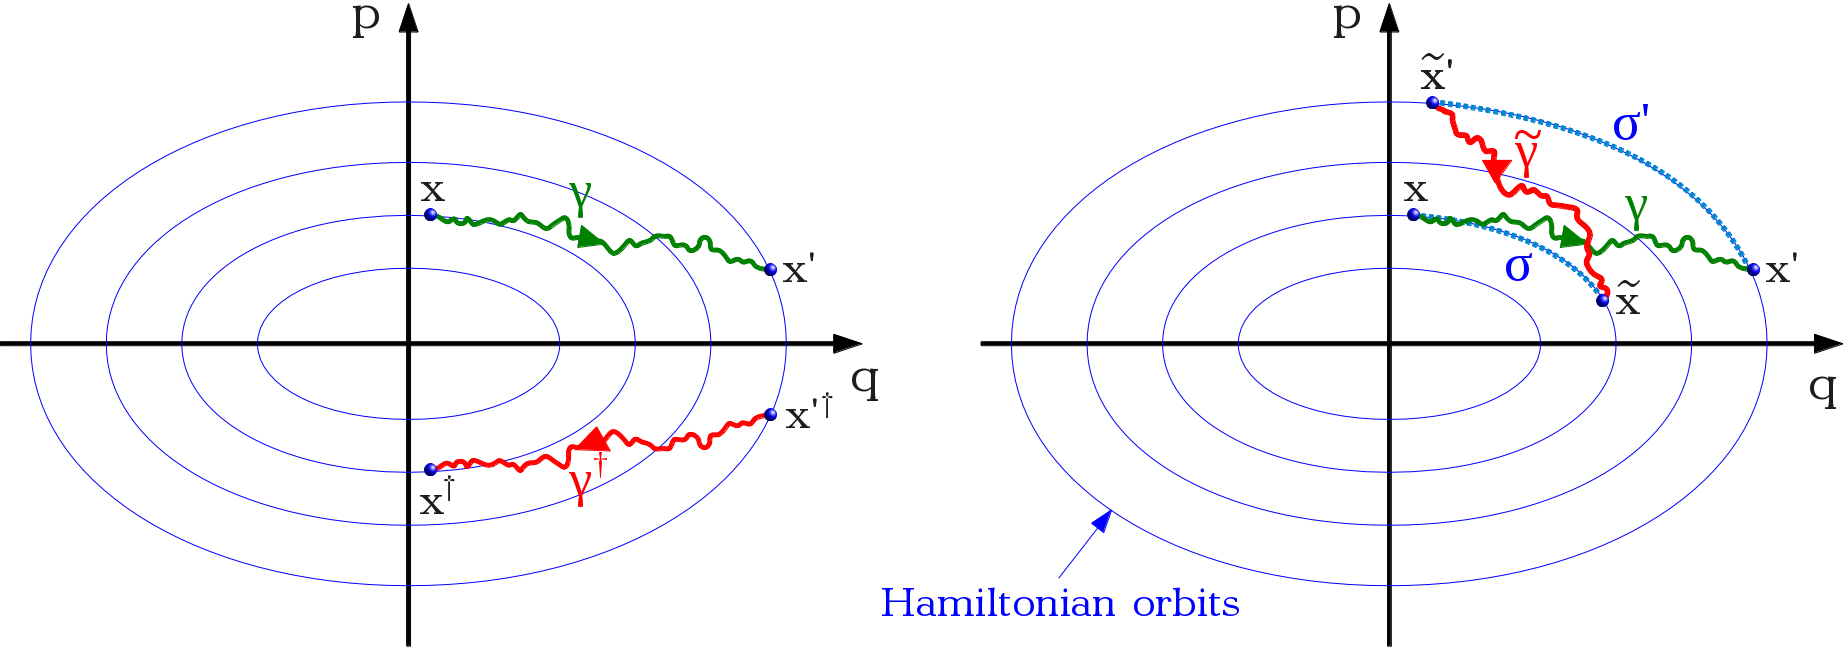
\includegraphics[width=0.9 \linewidth]{figures/trajectories}
	\caption[]{Path construction in the two models. The left side shows SF's approach, which mirrors the forward trajectory \(\gamma\) into a different part of phase space (yielding \(\gamma^\dagger\)), and calculates the ratio of the weights of these two paths. On the right hand side is the flow-based approach, which does not mirror momenta; instead, it traces the Hamiltonian flow in order to reach the start and end points of the conjugate process \(\tilde\gamma\). (Image by Haye Hinrichsen, taken from \cite{flow-paper}.)}
	\label{fig:hf sf}
\end{figure}

%%%%%%%%%%%%%%%%%%%%%%%%%%%%%%%%%%%%%%%%%%%%%%%%%%%%%%%%%%%%%%%%%%%%%%%%%%%%%%
\subsection{Differences between the models}
%%%%%%%%%%%%%%%%%%%%%%%%%%%%%%%%%%%%%%%%%%%%%%%%%%%%%%%%%%%%%%%%%%%%%%%%%%%%%%


At this point may be a good idea to mention figure~\RefFigure{fig:hf sf} again, where the two path constructions (SF and flow) are pictured alongside each other. Important consequences compared to SF's model are as follows:
%
\begin{itemize}
	\item The \HF{} entropy definition is local in phase space: nothing is mirrored into a different part of phase space, and the entire quotient is constrained to an arbitrarily small part of phase space for sufficiently small timespans.
	\item Inside the \HF{} entropy definition, distinction between odd and even variables is necessary, again because of the absence of time or momentum reversal.
	\item No differential entropy is produced for ``transitioning'' onto the same orbit again in the \HF{} case, whereas for \SF{} this is not necessarily so.
\end{itemize}

The second point is particularly important, as it contains what is probably the crucial conceptual difference between \HF{} and \SF{}. For \HF{}, the splitting is done \emph{a priori} with only the equations of motion known, in particular before entropy is even mentioned. On the other hand, in Spinney/Ford's case, reversal of dynamics is hard-wired into the entropy definition itself. In other words, \textbf{the \HF{} approach factors out the reversal of dynamics}.

In order to obtain the conjugate propagator to the original forward process in the \HF{} model, the Hamiltonian part of the equations of motion needs to be known, which allows tracing the Hamiltonian flow back along the deterministic trajectory to reach the starting position of the reverse process, and similarly for the end position. In other words, the equations of motions must be partitioned in two parts, one for the Hamiltonian flow and one for the non-Hamiltonian processes such as dissipation and friction.

The principle behind the algorithm for the separation is inspired by the definition of the Riemann tensor: the system is run in a process that should return to the origin in the end; if it does not, the discrepancy is characteristic for a certain property of that system. In case of the Riemann tensor that discrepancy is the curvature of space, in phase space system it accounts for the non-Hamiltonian parts of the dynamics.

Formally, the most general equations of motion read, with \(x\) = \(q\) or \(p\):
%
\begin{align}
	\dot x &= f_x(q,p) + \Gamma_x(q,p)\xi_x(t)
\end{align}
%
This can be split up in Hamiltonian (\(\dot x_H\)) and non-Hamiltonian (\(\dot x_\Delta\)) parts:
%
\begin{align}
	\dot x &= \dot x_H + \dot x_\Delta
\end{align}
%
To obtain the summands individually, the following algorithm is used:
%
\begin{enumerate}
	\item Calculate \(x(t+\d t/2) \).
	\item Reverse the system's dynamics by substituting \(p \to -p\).
	\item Evolve the for another \(\d t/2\), starting at the previously reached end point.
	\item The end position is \(x(t+\d t)\), from which \(x_\Delta = x(t+\d t) - x(t)\) can be determined.
\end{enumerate}
%
For example, this procedure applied to the underdamped particle discussed in the present work
%
\begin{align*}
	\dot q &= p \\
	\dot p &= -V'(q) - \mu(p)p + \Gamma(p)\xi(t)
\end{align*}
results in
\begin{align*}
	\dot q_H &= p  &  \dot q_\Delta &= 0 \\
	\dot p_H &= -V'(q)  &  \dot p_\Delta &= - \mu(p)p + \Gamma(p)\xi(t) ~.
\end{align*}
This approach is quite general and can be applied to more complicated systems, in which the separation may not be as clear.



%%%%%%%%%%%%%%%%%%%%%%%%%%%%%%%%%%%%%%%%%%%%%%%%%%%%%%%%%%%%%%%%%%%%%%%%%%%%%%
\subsection{Flow-based entropy production of the model}
%%%%%%%%%%%%%%%%%%%%%%%%%%%%%%%%%%%%%%%%%%%%%%%%%%%%%%%%%%%%%%%%%%%%%%%%%%%%%%

This new model can now be applied to the one-dimensional underdamped particle introduced before in section~\RefSection{sec:underdamped-model}. Here, the forward process starts at \(\vec x = (q,p)\) and ends at \(\vec x' = (q',p')\). The conjugate process starts at \(\tilde{\vec x}' = (q'-p'\d t, p'-f(q')\d t)\), which as described before is where tracing back the Hamiltonian orbit through \((q',p')\) for a timespan \(\d t\) reaches; similarly, \(\tilde{\vec x} = (q+p\d t, p+f(q)\d t)\). The entropy thus reads
%
\begin{equation}
	\label{eqn:flow entropy quotient}
	\d\SEnv^\HF(\vec x'|\vec x;\,\d t)
	= \lim_{\varepsilon\to0}
		\frac{
			_\varepsilon G_a(q',p'|q,p;\,\d t)
		}{
			_\varepsilon G_b(q+p\d t, p+f(q)\d t)|q'-p'\d t, p'-f(q')\d t;\,\d t)
		}
\end{equation}
%
where the propagator has no explicit \(t\) dependence, which has therefore been dropped in the notation. The same argument that has been made in the SF case in \RefEqn{eqn:delta-limit} -- namely that in the limit \(\varepsilon\to0\) the location has to behave deterministically, giving a condition on the ambiguity parameters \(a\) and \(b\) -- can be used here to yield
%
\begin{equation}
	\begin{split}
	&(q'-q)-\bigl(p+a(p'-p)\bigr)\d t
	\\=&
	-\Bigl( (q-q')+(p+p')\d t \\
	&\qquad - \bigl( p'-f(q')\d t + b(p-p'+(f(q)+f(q'))\d t)\bigr) \Bigr)
	\end{split}
\end{equation}
%
which holds iff \(a = b = \tfrac12\), as can be shown by expanding the force \(f(q')\) around \(q\) and neglecting terms of \(\Cal O(\d t^3)\). This makes a lot of sense, as it means that the fields are evaluated around the center of each trajectory, which to leading order in time is the same for both processes. This result is much stronger than what is obtained in SF's case, where \(a = b\) is imposed, without giving them a specific value.

Like in the SF chapter before, the entropy production \RefEqn{eqn:flow entropy quotient} can be calculated in this case, yielding \TODO{verify}
%
\begin{equation}\begin{split}
	\label{eqn:hf entropy}
	\d\SEnv^\HF &=
	\frac1{\Gamma^2}\bigl(-2p\mu V'-2\Gamma\Gamma'V'\bigr)\d t
	+ \frac1{\Gamma^2}\bigl(-2p\mu-2\Gamma\Gamma'\bigr)\d p
	\\&\qquad
	+ \frac1{\Gamma^2}\bigl( -p\mu' + 2p\mu \tfrac{\Gamma'}\Gamma - \mu - \Gamma\Gamma'' + \Gamma'^2 \bigr) \d p^2
	\\&\qquad
	+ \Cal O(\d t^2) + \Cal O(\d p^3)
\end{split}\end{equation}
%
where once again the explicit dependencies of the coefficients have been dropped for brevity. This result shows some important differences compared to SF's result \RefEqn{eqn:sf entropy production}:
%
\begin{itemize}
	\item No entropy is produced to leading order in \(\d t\) along the deterministic trajectory \(\d p = -V'(q)\d t\). This is of course a direct result of the construction, which specifically addressed the issue that only switching orbits should yield an entropy contribution.
	\item While the SF result does not include a term proportional to \(\d p^2\), the expression here does.
	\item Applied to a particle in a system with linear friction and additive noise in detailed balance, the expression reduces to the expected textbook result \RefEqn{eqn:classical environmental entropy production}.
	\item The result coincides with the result SF would have gotten, had they not chosen \(a = \tfrac12\) instead of \(0\) in their model -- \RefEqn{eqn:sf entropy production 1/2} is identical to \RefEqn{eqn:hf entropy}! This brings up the question once again as to why they made this specific choice, but as mentioned earlier, this is done without further comment in \cite{sf}.
\end{itemize}






%%%%%%%%%%%%%%%%%%%%%%%%%%%%%%%%%%%%%%%%%%%%%%%%%%%%%%%%%%%%%%%%%%%%%%%%%%%%%%
\section{Towards observable quantities}
%%%%%%%%%%%%%%%%%%%%%%%%%%%%%%%%%%%%%%%%%%%%%%%%%%%%%%%%%%%%%%%%%%%%%%%%%%%%%%

The previously defined quantity \(\d\SEnv(\vec x'|\vec x;\,\d t)\) is a two-point function, yielding the expected entropy production for the transition \(\vec x\to\vec x'\). However, this quantity is not easily accessible by experiment or simulation: while the starting point \(\vec x\) can be set, \(\vec x'\) is much less accessible due to it being statistically distributed over arbitrary phase space regions. The following sections will successively integrate out the unknowns, in order to yield a testable result.


%%%%%%%%%%%%%%%%%%%%%%%%%%%%%%%%%%%%%%%%%%%%%%%%%%%%%%%%%%%%%%%%%%%%%%%%%%%%%%
\subsection{Local entropy production}
%%%%%%%%%%%%%%%%%%%%%%%%%%%%%%%%%%%%%%%%%%%%%%%%%%%%%%%%%%%%%%%%%%%%%%%%%%%%%%

\newcommand\SEnvLoc{\ensuremath{S_\text{env,\,loc}}}

The \emph{local entropy production rate} integrates out the final phase space coordinate:
%
\begin{equation}
	\d\SEnvLoc(\vec x;\,\d t) = \int_\Omega\d\vec x' G_c(\vec x'|\vec x;\,\d t) \d\SEnv(\vec x'|\vec x;\,\d t) + \Cal O(\d t^2)
\end{equation}
%
This describes the expected change in environmental entropy in a short timespan \(\d t\), given an initial location \(\vec x\) in phase space \(\Omega\). Note that the propagator to encode the transition likelihood contains yet another ambiguity parameter in addition to \(a\) and \(b\) implicitly contained in \(\d\SEnv\).

Translated to the present model of a particle in two-dimensional phase space, the equation reads
%
\begin{equation}\begin{split}
	\label{eqn:local entropy 1d}
	\d\SEnvLoc(q,p;\,\d t) &= \inflint\d q'\inflint\d p'\; G_c(q',p'|q,p;\,\d t) \d\SEnv(q',p'|q,p;\,\d t)
	\\&\quad + \Cal O(\d t^2) ~.
\end{split}\end{equation}
%
To calculate its value, first expand the ordinary differential entropy production in terms of differences of its arguments,
%
\begin{equation}
	\label{eqn:dSEnv power expansion}
	\d\SEnv(q',p'|q,p;\,\d t)
	= \sum_{i,j=0}^\infty
	\sigma_{ij}(q,p,\d t)
	(q'-q)^i
	(p'-p)^j
	+ \Cal O(\d t^2)
\end{equation}
%
so that \(\sigma_{ij}\) are the Taylor coefficients of \(\d\SEnv\) in terms of \(q\) and \(p\). Inserting this expansion in \RefEqn{eqn:local entropy 1d} yields
%
\begin{equation}\begin{split}
	\d\SEnvLoc(q,p;\,\d t) &=
	\sum_{i,j=0}^\infty
	\sigma_{ij}(q,p,\d t)
	\\&\qquad
	\times\inflint\d q'
	\inflint\d p'
	\; G_c(q',p'|q,p;\,\d t)
	(q'-q)^i
	(p'-p)^j
	\\&\qquad + \Cal O(\d t^2)
\end{split}\end{equation}
%
where the second line can be identified as the \((i,j)\)-th \((q,p)\) propagator moments respectively,
%
\begin{equation}
	M_{ij,c}(q,p,\d t) = 
	\inflint\d q'
	\inflint\d p'
	\; G_c(q',p'|q,p;\,\d t)
	(q'-q)^i
	(p'-p)^j
\end{equation}
%
which allows rewriting \(\d\SEnvLoc\) as
%
\begin{equation}
	\label{eqn:dSEnvLoc split up}
	\d\SEnvLoc(q,p;\,\d t)
	=
	\sum_{i,j=0}^\infty
	\sigma_{ij}(q,p,\d t)
	M_{ij,c}(q,p,\d t)
	+ \Cal O(\d t^2)
\end{equation}
%
where the expression is split up in two parts that easily combine into the local entropy production: \(\sigma_{ij}\) is obtained via the expansions of the known propagator quotients from the previous section using \RefEqn{eqn:dSEnv power expansion}, and the not yet known propagator moments \(M_{ij,c}\).



In the case of the present model of the underdamped particle \RefEqn{eqn:underdamped sde epsilon}, the propagator moments can be calculated. Due to the length of the intermediate results, this calculation can be found in appendix~\RefSection{sec:fp moments}. The result obtained there is
%
\begin{align}
	M_{00;c} &= 1 + \Cal O(\d t) \\
	M_{01;c} &= (-p\gamma(p) - V'(q)) \d t + \Cal O(\d t^2) \\
	M_{02;c} &= \Gamma(p)^2 \d t + \Cal O(\d t^2) \\
	M_{ij;c} &= \Cal O(\d t^{i+1}) \quad (i,j > 0)
\end{align}
%
These expressions are noteworthy in a couple of ways:
\begin{enumerate}
	\item The ambiguity parameter \(c\) does not appear in terms of leading order, indicating that the propagator moments are independent of said ambiguity at least in the present special case, where the fields are evaluated linearly between start and end points. (Recall that the most general version, introduced in section~\RefSection{sec:general propagator case}, allows evaluation at arbitrary points \(\varphi(\vec x,\vec x')\), whereas here \((1-c)\vec x + c\vec x'\) has been chosen.)
	\item None of the nonzero \(\d q\) moments matter; they all contribute to higher-order in \(\d t\) terms only.
	\item The ad-hoc quantity \(\varepsilon\) of the equations of motion \RefEqn{eqn:underdamped sde epsilon} vanishes naturally in the calculation, once again justifying its previous introduction.
\end{enumerate}

Now \(\d\SEnvLoc\) can be calculated for the Spinney-Ford case with \(a=0\), the Hamiltonian Flow model and therefore also \SF with \(a = \tfrac12\), and remarkably the results are all identical, namely \TODO{verify formula}
%
\begin{equation}\begin{split}
	\d\SEnvLoc(q,p,\d t)
		&=
		\Bigl(-\mu(p) - p \mu'(p) + \frac{2p^2\mu(p)^2}{\Gamma(p)^2} + \frac{4p\mu(p)\Gamma'(p)}{\Gamma(p)} \\
		&\qquad + \Gamma'(p)^2 - \Gamma(p)\Gamma''(p)\Bigr) \, \d t + \Cal O(\d t^2) ~.
\end{split}\end{equation}
%
The terms proportional to \(\d p^2\) in \RefEqn{eqn:hf entropy} compensate the other differences compared to \RefEqn{eqn:sf entropy production} during integration (i.e. multiplication with the propagator moments) by moving them to higher orders of \(\d t\), explaining how different differential entropies can yield the same local entropy production.





%%%%%%%%%%%%%%%%%%%%%%%%%%%%%%%%%%%%%%%%%%%%%%%%%%%%%%%%%%%%%%%%%%%%%%%%%%%%%%
\subsection{Global entropy production}
\label{sec:global entropy production}
%%%%%%%%%%%%%%%%%%%%%%%%%%%%%%%%%%%%%%%%%%%%%%%%%%%%%%%%%%%%%%%%%%%%%%%%%%%%%%

The \emph{global entropy production} once again averages over all positions, to give an expectation value for the short-time environmental entropy production in an ensemble of many (non-interacting) particles. It is obtained from the local entropy production developed just above via
%
\begin{equation}\begin{split}
	\label{eqn:global entropy production}
	\langle\d\SEnv\rangle(t)
	&= \d t \int_\Omega \d\vec x P(\vec x, t)\d\SEnvLoc(\vec x, \d t) \\
	&= \d t \infint\!\!\d q\infint\!\!\d p\, P(q, p, t) \, \d\SEnvLoc(q, p, \d t)
\end{split}\end{equation}
%
where \(P\) is the probability density for being in a certain point of phase space.

For example, take a system in thermal equilibrium. Here, \(\mu(p)\) and \(\Gamma(p)\) are related via the generalized Einstein relation \RefEqn{eqn:einstein}, and \(P(q,p)\) is Boltzmannian. The differential entropy productions then turn out to be
%
\begin{align}
	\d\SEnv^\SF &= -\beta p(\d p + V'(q)\d t) - \frac\beta2\Gamma(p)^2 + \Cal O(\d t^2) + \Cal O(\d p^3) \\
	\d\SEnv^\HF &= -\beta p(\d p + V'(q)\d t) + \Cal O(\d t^2) + \Cal O(\d p^2)
\end{align}
%
which also showcases the previously claimed fact that \SF's result does not vanish along the deterministic trajectory \(\d p = -V'(q)\d t\), while the \HF{} result does. Maybe more importantly even, \SF's result does not reproduce the result previously obtained using only classical thermodynamics in \RefEqn{eqn:classical environmental entropy production}. However, as claimed earlier, the resulting local entropy production is identical for both results,
%
\begin{equation}
	\d\SEnvLoc(q,p,\d t) = \left(
		- \tfrac12\beta\Gamma(p)^2
		+ \tfrac12\beta^2p^2\Gamma(p)^2
		- \beta p\Gamma(p)\Gamma'(p)
		\right)\,\d t
		+ \Cal O(\d t^2) ~.
\end{equation}
%
By integrating this together with the Boltzmann distribution
%
\begin{equation}
	P(q,p) = \frac1Z e^{-\beta\left(\frac{p^2}2-V(q)\right)}
\end{equation}
%
in \RefEqn{eqn:global entropy production}, the global entropy production can be obtained. As the explicit calculation in appendix~\RefSection{sec:global entropy zero} shows, the result is
%
\begin{equation}
	\label{eqn:global entropy 0}
	\forall t. ~ \langle\d\SEnv\rangle(t) = 0
\end{equation}
%
which is what a system obeying detailed balance in thermal equilibrium should obey. This is in agreement with classical thermodynamics again, and the necessity for the previous calculation also hints at why the expression for \(\d\SEnv\) in \RefEqn{eqn:classical environmental entropy production} is not entirely correct: although it assumes \emph{some} properties equilibrium provides, it is a ``thermodynamic'' quantity in terms of \(q\) and \(p\), while classical thermodynamics only deals with averages in which single appearances of location and momentum are meaningless.


%%%%%%%%%%%%%%%%%%%%%%%%%%%%%%%%%%%%%%%%%%%%%%%%%%%%%%%%%%%%%%%%%%%%%%%%%%%%%%
\section{Conclusion}
%%%%%%%%%%%%%%%%%%%%%%%%%%%%%%%%%%%%%%%%%%%%%%%%%%%%%%%%%%%%%%%%%%%%%%%%%%%%%%

Although the initial goal of the presented subject was finding a better definition of entropy production in continuous settings, it turned out that both the new (flow based) and the old (SF, \cite{sf}) approach yield identical results both for the local and the global environmental entropy production in the scenarios presented above. This leads to the conclusion that (two-point) \textbf{short-time environmental entropy production is not a uniquely defined quantity}, and should be regarded as a mathematical intermediate step. However, the flow-based approach seems to be closer to physical intuition, as it does not require a time reversal (which is particularly difficult to map to the real world), its intermediate results vanish along the deterministic trajectory of the system, the distinction between odd and even variables is not necessary, and the propagator ambiguities fall away during the calculation without making further assumptions (which is important to mention because SF and HF models are identical in their two-point entropy production, given the \emph{arbitrary} choice of \(a = \tfrac12\) in the former model).

It is worth noting that the case of a more general system than \RefEqn{eqn:model hamiltonian eqns of motion} has not been investiated, and it is unknown whether both path constructions still agree in this scenario. Furthermore, the SDE of the system has been integrated according to the \Ito{} scheme in order to obtain the FP equation; the consequences of choosing Stratonovich or an arbitrary parameter value for the stochastic integration are also subject to further research.






\appendix
\chapter{Appendix}

\section{Calculation of Fokker-Planck propagator moments}

The following describes how to calculate the \((i,j)\)-th \((\d q, \d p)\) moment of the Fokker-Planck (FP) propagator. For the system discussed in this thesis \TODO{ref to eqn of motion} \TODO{ref to paper}, it has the rather long form

\begin{align*}
	&G_a(q,p,\d q,\d p,\d t) = \\
	& \frac1{2 \pi  \d t \varepsilon  \Gamma (a \d p +p)}
	  ~\exp \Bigl(\frac1{2 \d t} \\
	%
	&\quad \Bigl(
		-\frac{(\d q-\d t (a \d p +p))^2}{\varepsilon ^2} \\
		&\qquad +\frac{\left(\d t (a \d p +p) \gamma (a \d p +p)+2 a \d t  \Gamma (a \d p +p) \Gamma '(a \d p +p)+\d p+\d t v'(a \d q+q)\right)^2}{\Gamma (a \d p +p)^2} \\
		&\qquad +2 \d t^2 a  \left(-(a \d p +p) \gamma '(a \d p +p)-\gamma (a \d p +p)\right) \\
		&\qquad -2 \d t^2 a ^2 \left(\Gamma (a \d p +p) \Gamma ''(a \d p +p)+\Gamma '(a \d p +p)^2\right)\Bigr)\Bigr)
\end{align*}

In the following, a modified version of the method of steepest descent will be derived, and then applied to the propagator to calculate the moments up to the needed order.


\subsection{Generalized method of steepest descent}

The moments of the FP propagator can be calculated similar to how the method of steepest descent is derived. However, there are a few details making it a little more difficult:

\begin{enumerate}
	\item The standard formula for steepest descent assumes that the exponential's prefactor is independent of the ``small'' quantity. This is not the case for the FP propagator, so a new formula has to be developed, albeit in the same spirit.
	\item Terms quickly grow with increasing order. While it must be made sure that no significant terms are omitted, calculating ``too much'' and dropping unnecessary terms afterwards introduces a lot of work and potential oversights. For that reason one should very carefully keep track of the orders of the terms to be calculated; the criteria for this turn out to be quite different in each order.
\end{enumerate}


\subsection{i-th dq moment}

Calculation of the \(i\)-th \(\d q\) moment is a straightforward application of the method of steepest descent

\subsection{j-th dp moment}

\begin{thebibliography}{99}
	\bibitem{thingie-paper} {
		D. Luposchainsky, A. Barato, H. Hinrichsen \\
		Phys. Rev. E 87, 042108 (2013) \\
		\emph{Strong fluctuation theorem for nonstationary nonequilibrium systems}
		}
	\bibitem{flow-paper} {
		D. Luposchainsky and H. Hinrichsen \\
		\TODO{update with JSP ref} \\
		\emph{Entropy production in continuous phase space systems}
		}
	\bibitem{seifert-review} {
		U. Seifert \\
		Rep. Prog. Phys. 75 126001 \\
		\emph{Stochastic thermodynamics, fluctuation theorems and molecular machines}
		}
	\bibitem{sf} {
		R.~Spinney and I.~Ford \\
		Phys. Rev. E 85, 051113 (2012) \\
		\emph{Entropy production in full phase space for continuous stochastic dynamics}
		}
	\bibitem{sde} {
		L. Evans \\
		Lecture notes on mathematics \\
		\emph{An Introduction to Stochastic Differential Equations}
		}
	\bibitem{sengupta} {
		A. Sengupta \\
		Summer term 2012 at Rutgers/USA \\
		\emph{Lecture notes on theoretical biophysics}
		}
	\bibitem{wissel} {
		C. Wissel \\
		Z. Phys. B 35, 185 (1979) \\
		\emph{Manifolds of equivalent path integral solutions of the Fokker-Planck equation}
		}
	\bibitem{donoso} {
		J. Donoso, J. Salgado, M. Soler \\
		J. Phys. A: Math. Gen. 32 (1999) 3681-3695 \\
		\emph{Short-time propagators for nonlinear Fokker-Planck equations}
		}

		
\end{thebibliography}


\end{document}